%% ─────────────────────────────────────────────────────────────────
%% PREAMBLE
%% ─────────────────────────────────────────────────────────────────
\documentclass[a4paper,fleqn,nologo]{cas-dc}

\usepackage[authoryear]{natbib}
\usepackage{amsmath}      % displaystyle, equations
\usepackage{booktabs}     % \toprule, \midrule, \bottomrule, \cmidrule
\usepackage{subcaption}   % subfigure environment
\usepackage{threeparttable} % tablenotes environment
\usepackage{placeins}     % \FloatBarrier to keep floats within sections
\usepackage{float}        % [H] placement specifier
\usepackage{longtable}    % multi-page tables
\usepackage[utf8]{inputenc}
\usepackage[T1]{fontenc}

%% ─────────────────────────────────────────────────────────────────
\begin{document}
\let\WriteBookmarks\relax
\def\floatpagepagefraction{1}
\def\textpagefraction{.001}

%% ── Metadata ─────────────────────────────────────────────────────
\shorttitle{DQI: Damage Detection in Jacket Offshore Platforms}
\shortauthors{Cisneros-Ruiz et al.}

\title[mode = title]{%
  Detection Quality Index (DQI): Inverse Optimisation Methodology
  Based on Genetic Algorithms for Damage Identification
  in Jacket-Type Offshore Platforms}

%% ── Author 1 ─────────────────────────────────────────────────────
\author[1]{Francisco~Javier Cisneros-Ruiz}[orcid=0009-0005-7017-4027]
\cormark[1]
\ead{fcisnerosr@outlook.es}
\credit{Conceptualization, Methodology, Software, Formal analysis, Writing -- Original Draft}
\affiliation[1]{
    organization={Postgraduate Program, Instituto Mexicano del Petroleo},
    addressline={Eje Central Lazaro Cardenas Norte 152},
    city={Mexico City},
    country={Mexico}
}

%% ── Author 2 ─────────────────────────────────────────────────────
\author[2]{Ivan Felix-Gonzalez}
\credit{Supervision, Writing -- Review \& Editing}
\affiliation[2]{
    organization={Instituto Mexicano del Petroleo},
    addressline={Eje Central Lazaro Cardenas Norte 152},
    city={Mexico City},
    country={Mexico}
}

%% ── Author 3 ─────────────────────────────────────────────────────
\author[3]{Rolando Salgado-Estrada}
\credit{Supervision, Writing -- Review \& Editing}
\affiliation[3]{
    organization={Facultad de Ingenier\'{i}a de la Construcci\'{o}n y el H\'{a}bitat,
                  Universidad Veracruzana},
    city={Veracruz},
    country={Mexico}
}

\cortext[1]{Corresponding author}

%% ── Abstract & Keywords ──────────────────────────────────────────
\begin{abstract}
The aging of offshore oil infrastructure and the high costs and risks
associated with traditional underwater inspections demand new integrity
management strategies. This paper proposes a Structural Health Monitoring
(SHM) methodology based on inverse optimisation using Genetic Algorithms
(GA) for damage identification in Jacket-type platforms. The Detection
Quality Index (DQI) is introduced as a new objective metric designed to
fuse multiple vibration-based indicators and mitigate numerical uncertainty by
penalising false positives. Validation was conducted over 3{,}240
simulation runs on a calibrated finite-element model under corrosion and
denting scenarios. Quantitative results demonstrate a differentiated
structural behaviour: secondary elements (braces) act as ``structural
fuses'', detectable from 30\% damage severity with global detection rates
of 92.2\% (denting) and 96.5\% (corrosion), while main elements (legs)
require severity levels exceeding 50\%. A novel Topology-Weighted
Precision metric is also proposed, correcting systematic underestimation
of localisation quality by the classical Precision metric, yielding gains
of up to $+$22 percentage points for brace elements.
\end{abstract}

\begin{keywords}
  Structural Health Monitoring \sep
  Genetic Algorithms \sep
  Jacket Platforms \sep
  Detection Quality Index \sep
  Inverse Optimisation \sep
  Topology-Weighted Precision
\end{keywords}

\begin{highlights}
\item A Detection Quality Index (DQI) fusing eight vibration-based indicators with exponential false-positive penalisation improves damage detection reliability in noisy offshore environments.
\item Secondary elements (braces) behave as structural fuses, detectable from 30\% severity, achieving 92.2\% (denting) and 96.5\% (corrosion) global detection rates.
\item Main elements (legs) require damage severity exceeding 50\% for reliable detection, indicating strong structural redundancy.
\item A Topology-Weighted Precision metric corrects classical Precision underestimation by up to $+$22 percentage points for brace elements in jacket lattice structures.
\item Validated over 3{,}240 simulation runs on a calibrated finite-element model under corrosion and denting scenarios, with AUC-ROC $>$\,0.90 for brace and inclined-leg members.
\end{highlights}

\maketitle

%% ── Spanish abstract (for informational purposes, omitted in submission) ────

\section{Introduction}

The global energy transition and the mounting pressure on offshore asset operators to extend the service life of their installations have elevated structural integrity management to a strategic priority of the highest order \citep{hlaing2024lifecycle}. Jacket-type platforms, characterised by their three-dimensional steel lattice configuration, form the backbone of hydrocarbon production facilities in shallow and intermediate waters, and are playing an increasingly important role as foundations for offshore wind turbines \citep{mdpi2024shm_wind}. These structures must simultaneously withstand production deck loads, stochastic hydrodynamic forces from waves and currents, and, in the case of wind turbines, the inertial forces transmitted from the nacelle and blades. In strategic regions such as the Gulf of Mexico, a significant proportion of fixed infrastructure has exceeded its original design service life---typically 20 to 25 years---and continues to operate under conditions of accelerated corrosion-induced and fatigue-driven deterioration \citep{mubarak2020condition}. Historically, the integrity management of these structures has relied on periodic visual inspections conducted by industrial divers or remotely operated vehicles (ROVs), methods that not only entail exorbitant operational costs and significant personnel risks \citep{instituto2020tech}, but are systematically inadequate for detecting internal or localised damage at early stages---a limitation further compounded by sector-wide maintenance budget cuts.

\section{Literature Review}

The marine environment subjects jacket structures to a convergence of degradation mechanisms of stochastic and electrochemical nature that simultaneously compromise their strength and dynamic response. Corrosion, exacerbated by salinity, humidity, and seawater temperature variations, does not act uniformly along the structure: integrity studies in tropical environments document corrosion rates in the Splash Zone of between 0.28 and 0.35~mm/year---values 140\% to 175\% higher than those assumed in the original design---with localised pitting of up to 4.8~mm recorded over as little as 18 months of operation \citep{birci2020integrity}. This cross-sectional loss raises the Unity Check (UC) utilisation ratio---the ratio of acting stress to member resistance capacity---whose critical operational threshold is UC~$=~0.8$ in accordance with current structural integrity guidelines \citep{API2014_manual, salama2020shm}. Simultaneously, marine growth accumulation on tubular members increases their effective hydrodynamic diameter, amplifying drag forces according to the Morison equation and shifting the natural frequencies of the structure in a way that can mask modal changes caused by stiffness loss \citep{salama2020shm}. These mechanisms are compounded by fatigue cracking, driven by the cyclic nature of wave loading and operational vibrations, which initiates preferentially at the weld toe of tubular joints in T, K, and Y configurations---high stress concentration points---and propagates silently with globally imperceptible stiffness changes for distributed sensor networks \citep{raza2021fatigue}.

In response to these limitations, Structural Health Monitoring (SHM) has undergone a paradigm shift since 2018, migrating from periodic inspections towards real-time diagnostic systems based on vibration response and artificial intelligence \citep{ghsoub2018structural, mdpi2024shm_wind}. Vibration-based damage identification exploits the physical relationship between modal properties---natural frequencies and mode shapes---and the structural stiffness state: a local stiffness reduction modifies global modal properties in a way that, in principle, can be inverted to localise and quantify damage. This approach is formalised as a model updating problem: given experimental modal parameters, the finite-element model parameters are calibrated to minimise the discrepancy between simulated and measured responses \citep{doebling1996damage}. However, the solution to this inverse problem is inherently ill-conditioned---non-unique and sensitive to perturbations---when attempting to parametrically adjust a structure with hundreds of members from a limited number of experimentally identified modes, frequently leading to physically inconsistent solutions \citep{aghaeidoost2023generalized}.

The most advanced model updating methodologies, proposed between 2022 and 2024, address this high-dimensionality problem through sensitivity-based clustering, which categorises structural members into homogeneous groups of dynamic behaviour to reduce the effective number of parameters to be optimised \citep{jiang2024model}. Natural frequency error and modal shape discrepancy are simultaneously adopted as objective functions, with the latter evaluated through the Modal Assurance Criterion (MAC), whose unit value indicates perfect vector correlation between the experimental and numerical eigenvectors \citep{jiang2024model}. Solving both error functions concurrently constitutes a multi-objective optimisation problem for which gradient-based methods are unsuitable given the model non-linearity and multiplicity of local minima.

In this context, Genetic Algorithms (GAs) have consolidated their position as the reference search engine for inverse optimisation in offshore SHM \citep{goldberg1989genetic}. Their principal advantage lies in the capacity to explore high-dimensional solution spaces without requiring gradient information, while maintaining notable robustness against local minima and noisy input data. Previous research on jacket platforms has demonstrated that GAs can identify damage location and severity with estimation errors of 3\% to 5\% when modal data are contaminated with random noise of up to 3\%, validating their applicability under realistic offshore measurement conditions \citep{rahmani2013ga}. Nevertheless, the effectiveness of these algorithms depends critically on the objective function formulation: a function that fuses multiple damage indicators and effectively penalises false positives constitutes the key differentiating element for reliable diagnostic systems in offshore operations \citep{malekzadeh2013damage}.

An aspect that has received renewed attention since 2022 is the quantitative assessment of damage localisation quality. The classical Precision metric penalises all false positives (FPs) identically, regardless of their spatial proximity to the truly damaged element, which is inadequate in lattice structural networks where an adjacent FP (topological distance $d=1$) carries a radically different engineering interpretation from one at the opposite end of the structure. Recent work has proposed distance-weighted metrics---such as MASDWP (\textit{Mean Average Spatial Distance-Weighted Precision})---that provide a more accurate assessment of localiser performance in large-scale structures \citep{li2024reliability}. In parallel, the Spatio-Temporal Graph Machine Learning (TVML) framework characterises the sensor network through centrality metrics---\textit{TopoScore}---selecting representative nodes from each modal cluster to reduce instrumentation cost without sacrificing diagnostic fidelity \citep{ma2024tvml}.

The quantitative validation of these systems relies on standard classification metrics---Precision, Recall, and the area under the ROC curve (AUC-ROC)---which allow evaluation of the trade-off between true positive rate and false alarm cost independently of the decision threshold \citep{li2024reliability}. Despite this scientific maturity, a significant normative gap persists: current international standards---ISO~19902, API~RP~2SIM, DNV-RP-C210, and NORSOK~N-005---provide general integrity management guidelines without digital twins and automated damage detection having attained regulatory requirement status \citep{ramboll2022digital}.

The work most closely related to the present study is that of Ervin and Zeng \citep{ervin2022index}, who proposed combining multiple DIs through a GA and demonstrated that the optimal combination outperforms any individual indicator, achieving detection rates of 94\% for 60\% reductions in Young's modulus under 5\% noise conditions. However, their formulation employed a binary target vector and was validated on planar steel frames, without incorporating false-positive penalisation or addressing the hydrodynamic complexities, structural redundancy, and diversity of damage mechanisms (corrosion~+~denting) characteristic of offshore jacket platforms.

The state-of-the-art review thus reveals three technical gaps motivating the present research. First: the absence of a unified objective function that fuses multiple vibration-based indicators and exponentially penalises false positives, adapted to the noise conditions inherent to platforms in operation. Second: the lack of a localisation metric that corrects the systematic underestimation of diagnostic quality caused by classical Precision in structurally redundant lattice networks. Third: the absence of exhaustive statistical validation of the operational hypothesis positing differentiated behaviour between secondary elements (braces or diagonals) and primary elements (legs) of the lattice under progressive corrosion and denting damage. Table~\ref{tab:comparison_sota} summarises the positioning of this study relative to the two most closely related GA-based approaches.

\begin{table*}[!ht]
  \centering
  \small
  \caption{Comparative positioning of the proposed methodology relative to the most closely related GA-based SHM approaches. N/R: not reported in the referenced study.}
  \label{tab:comparison_sota}
  \begin{tabular}{lccc}
    \toprule
    \textbf{Aspect} & Rahmani \& Behzad & Ervin \& Zeng & \textbf{This study} \\
                    & \citep{rahmani2013ga} & \citep{ervin2022index} & \\
    \midrule
    Structure                            & Jacket platform        & Planar steel frame     & 3D 4-leg jacket        \\
    Damage mechanisms                    & Stiffness loss         & Stiffness loss         & Corrosion $+$ denting  \\
    Number of structural members         & N/R                    & N/R                    & 120                    \\
    Multiple DIs fused via GA            & No (model updating)    & Yes (75~DIs)           & Yes (8~DIs)            \\
    False-positive penalisation          & No                     & No                     & Yes (DQI)              \\
    Noise robustness validated           & 3\% noise              & 5\% noise              & SNR 5--50~dB           \\
    Statistical validation runs          & N/R                    & N/R                    & 3{,}240                \\
    Topology-weighted localisation metric& No                     & No                     & Yes (Precision$_w$)    \\
    \bottomrule
  \end{tabular}
\end{table*}

This study proposes an Inverse Optimisation strategy based on Genetic Algorithms for damage identification in jacket platforms. The central contribution is the \textbf{Detection Quality Index (DQI)}, a novel objective metric designed to fuse multiple damage indicators and exponentially penalise false positives, improving diagnostic reliability in noisy operational environments \citep{malekzadeh2013damage}. As a second methodological contribution, the \textbf{Topology-Weighted Precision} ($\text{Precision}_w$) is proposed, which assigns a weight $w(d) = d/(d+1)$ to each false positive as a function of its distance to the damaged element in the structural connectivity graph---a correction that, as demonstrated in Section~\ref{sec:resultados}, yields gains of up to $+22$~percentage points in localiser evaluation for braces. Validation was carried out over 3{,}240 algorithm runs on a calibrated finite-element model of a 4-leg jacket platform subjected to corrosion (5\%--90\% severity) and denting (5\%--45\%) scenarios, with quantitative analysis of Precision, Recall, and noise robustness via AUC-ROC (Section~\ref{subsec:SNR}).

The paper is organised as follows: Section~\ref{sec:modelado} describes the numerical modelling of the platform, incorporating added-mass and marine growth effects. Section~\ref{sec:metodologia} details the GA-based methodology and the mathematical formulation of the DQI. Section~\ref{sec:resultados} presents the results and discussion for the corrosion and denting scenarios, evaluating the sensitivity of the method. Finally, Section~\ref{sec:conclusiones} offers conclusions and future research directions.

\section{Numerical Modelling and Damage Formulation}
\label{sec:modelado}

The dynamic behaviour of the offshore platform is modelled by discretising the continuous structure into a multi-degree-of-freedom (MDOF) system. Under the assumption of linear elastic behaviour and small oscillations, the dynamic equilibrium is governed by the differential equation of motion for undamped free vibration:

\begin{equation}
    \label{eq:ec_movimiento}
    \mathbf{M}\ddot{\mathbf{u}}(t) + \mathbf{K}\mathbf{u}(t) = \mathbf{0}
\end{equation}

\noindent where $\mathbf{K}$ is the global stiffness matrix and $\mathbf{M}$ is the global mass matrix of the system ($n \times n$). The latter is critical in offshore structures, as it must incorporate not only the structural steel mass but also the complex hydrodynamic interactions described below.

\subsection{Components of the Global Mass Matrix}

To faithfully represent the physics of an in-service jacket platform, the mass matrix is assembled as the superposition of three components: structural mass ($M_s$), added mass ($M_a$), and trapped mass ($M_t$).

\subsubsection{Hydrodynamic Mass and Coefficients (\texorpdfstring{$C_m$}{Cm})}
The added mass represents the volume of fluid that oscillates in concert with the tubular member and is modelled through the mass coefficient $C_m$, which depends on surface roughness and biological fouling. In accordance with design practice and technical reports \citep{API2014_manual,CardenasArias2019_article}, reference values of $C_m=1.6$ for surfaces with significant marine growth and $C_m=1.2$ for clean surfaces are adopted in this study. Additionally, the trapped mass (water enclosed within flooded tubular cross-sections) is incorporated as internal added mass in the model assembly; experimental details and schematic descriptions of the definition and parametrisation of both terms are given in \citep{CardenasArias2019_article}.

\subsubsection{Marine Growth Modelling}

Marine growth modifies the effective mass and hydrodynamics of tubular members through variations in biological thickness along the water column; its impact depends on light exposure and depth \citep{birci2020integrity,salama2020shm}. In the numerical model, a variable thickness profile was implemented by vertical zones (tidal zone vs.\ seabed), locally adjusting the mass and inertia coefficients in the most affected regions.

\FloatBarrier
\subsection{Mechanics of Simulated Damage}

In contrast to black-box models, this research employs a physics-based approach to simulate damage. The geometric properties of the finite-element cross-sections are modified and the global matrices are re-assembled to obtain the updated modal properties (forward problem).

\subsubsection{Uniform Corrosion}
Corrosion is modelled as a uniform reduction of the wall thickness ($t$) of the tubular member over an affected length ($L_D$). This geometric loss reduces the cross-sectional area ($A$) and the moments of inertia ($I$), directly altering member stiffness. Regarding the elastic modulus ($E$), experimental studies by C\'{a}rdenas-Arias and Maldonado-Zepeda (2019) show that, in the linear elastic range, steel corroded by marine immersion does not exhibit significant changes in $E$; consequently, $E$ is held constant in this work and only geometric modifications ($A$, $I$) are considered for damage characterisation \citep{CardenasArias2019_article}.

\subsubsection{Denting}
Denting represents critical localised damage caused by accidental impacts. This damage is modelled by assuming a cross-sectional distortion that flattens the impacted face and widens the lateral surfaces, conserving the perimeter but drastically reducing the local moment of inertia ($I_{\text{red}}$) (Figure~\ref{fig:abolladura_seccion}).

\begin{figure}[!ht]
    \centering
    
\includegraphics[width=0.2\textwidth]{figs/004_modelo_elemento_tubula_seccion_longitudinal_parametros_abolladura.png}
    \caption{Parametrisation of the dented cross-section.}
    \label{fig:abolladura_seccion}
\end{figure}

To avoid abrupt numerical discontinuities in the stiffness matrix, the variation of inertia along the dented zone is smoothed through fourth-degree polynomial interpolation functions, ensuring a representative transition of local stiffness loss (Figure~\ref{fig:interpolacion_abolladura}).

\begin{figure}[!ht]
    \centering
    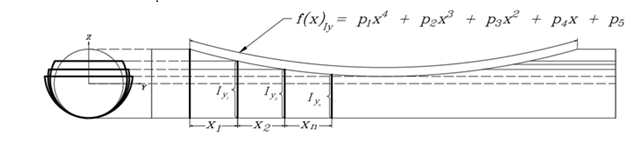
\includegraphics[width=0.9\columnwidth]{figs/004_modelo_elemento_tubular_seccion_longitudinal_parametros_abolladura_con_funciones_de_interpolacion.png}
    \caption{Longitudinal interpolation of moment of inertia in the dented zone for numerical smoothing.}
    \label{fig:interpolacion_abolladura}
\end{figure}

\subsection{Case Study: Jacket-Type Platform}

The methodology is validated on a numerical model of a fixed 4-leg jacket-type offshore platform, representative of structures installed in the shallow and intermediate waters of the Gulf of Mexico (Figure~\ref{fig:caso_estudio}). The three-dimensional geometry, section properties, and mass distribution were defined in commercial structural-analysis software (ETABS) and exported to a custom MATLAB framework that assembles the global mass and stiffness matrices and performs the modal, damage-simulation, and GA-optimisation analyses. The model comprises 120 structural elements and incorporates the complete superstructure and the pile foundation system (simulated via equivalent length to the apparent fixity point).

\begin{figure}[!ht]
    \centering
    % Isometric view only, enlarged
    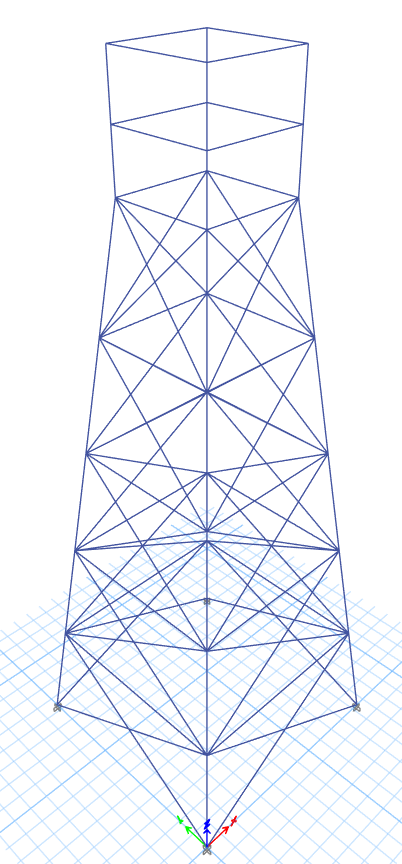
\includegraphics[width=0.4\columnwidth]{figs/007_modeo_vista_3d_de_plataforma_tipo_jacket_de_caso_de_estudio.png}
    \caption{Numerical model of the study platform: 3D isometric view.}
    \label{fig:caso_estudio}
\end{figure}


\section{Inverse Optimisation Methodology}
\label{sec:metodologia}

To address the structural damage identification problem in offshore platforms, this study extends the GA-based index combination framework proposed by Ervin and Zeng \citep{ervin2022index}, who demonstrated that a GA can optimally select and weight multiple individual damage indices (DIs), outperforming any single indicator. In the present work, that framework is adapted to the offshore jacket context and an original contribution is incorporated as the objective function: the Detection Quality Index (DQI), designed to exponentially penalise false positives and maximise diagnostic reliability in noisy environments---aspects not addressed in the original formulation of Ervin and Zeng \citep{ervin2022index}.

The methodology is fundamentally structured in two coupled stages: the mechanical simulation of damage scenarios and the stochastic optimisation of detection. The general operational workflow is detailed in Figure~\ref{fig:metodologia_general}. That figure illustrates the complete chain from data acquisition on the real platform to maintenance decision-making; the scope of the present work is confined to the central stage highlighted in the figure: numerical damage model generation, computation of the eight DIs, and DQI+GA optimisation for localisation of the affected member. In the context of inspection planning, Varela and Tolentino \citep{varela2023cost} note that structural review intervals for fixed platforms can reach up to six years under certain conditions; this observation is used here to contextualise the maintenance horizon considered in the operational recommendations derived from this study.

\begin{figure*}[!t]
    \centering
    
\includegraphics[width=0.9\textwidth]{figs/005_metogologia_propuesta_para_identificar_daños_en_plataformas_reales.jpg}
    \caption{General scheme of the proposed damage identification methodology. The delimited box indicates the scope of the present work: numerical simulation of damage scenarios, extraction of vibration-based indicators (DIs), and DQI+GA optimisation for localisation of the damaged member.}
    \label{fig:metodologia_general}
\end{figure*}

\subsection{Formulation of Vibration-Based Indicators}
Following the framework of Ervin and Zeng \citep{ervin2022index}, the detection system is fed by a set of damage indices (DIs) derived from the modal properties and flexibility matrix of the structure. Unlike the original work, which employs 51 uniaxial directional DIs and 24 triaxial resultant DIs, this study adopts eight scalar indicators representative of modal and flexibility changes, adapted to the three-dimensional jacket platform model. The mathematical formulations used as inputs to the GA are defined below, where $u$ denotes the undamaged state, $d$ the damaged state, $N_m$ the number of vibration modes considered in the analysis (in this study, $N_m = 6$, corresponding to the dominant global lateral-bending, rocking, and torsional modes of a four-leg jacket; this count is consistent with the number of modes reliably extractable from MEMS accelerometer arrays deployed on operating platforms \citep{ghsoub2018structural}), and $\mathcal{R}_j(\cdot)$ the extraction operator that selects the scalar value corresponding to the $j$-th structural element from the argument vector.

\subsubsection{Mode-Shape-Based Indicators}
\textbf{$DI_1$: COMAC} \\
COMAC quantifies the point-by-point correlation between two sets of mode shapes. The complement of its square root is employed for damage detection:
\begin{equation}
    \text{DI}_1(j) = 1 - \sqrt{ \frac{ \left( \sum_{i=1}^{N_m} |\phi_{u,ij}| |\phi_{d,ij}| \right)^2 }{ \sum_{i=1}^{N_m} \phi_{u,ij}^2 \sum_{i=1}^{N_m} \phi_{d,ij}^2 } }
\end{equation}

\textbf{$DI_2$: Absolute Mode Shape Difference} \\
Computes the magnitude of the change in the modal displacement vector:
\begin{equation}
    \text{DI}_2(j) = \mathcal{R}_j \left( \sum_{i=1}^{N_m} | \boldsymbol{\phi}_{u,i} - \boldsymbol{\phi}_{d,i} | \right)
\end{equation}

\textbf{$DI_3$: Relative Mode Shape Ratio} \\
Evaluates the deviation with a regularisation threshold $\epsilon = 10^{-6}$ (to avoid numerical division by zero):
\begin{equation}
    \text{DI}_3(j) = \mathcal{R}_j \left( \sum_{i=1}^{N_m} \left| \frac{\boldsymbol{\phi}_{d,i}}{\boldsymbol{\phi}_{u,i} + \epsilon} - 1 \right| \right)
\end{equation}

\subsubsection{Flexibility-Based Indicators}
The modal flexibility matrix is approximated as $\mathbf{F} \approx \boldsymbol{\Phi} \boldsymbol{\Omega}^{-2} \boldsymbol{\Phi}^T$.

\textbf{$DI_4$: Flexibility Difference} \\
\begin{equation}
    \text{DI}_4(j) = \mathcal{R}_j \left( | \text{diag}(\mathbf{F}_d) - \text{diag}(\mathbf{F}_u) | \right)
\end{equation}

\textbf{$DI_5$: Flexibility Ratio} \\
\begin{equation}
    \text{DI}_5(j) = \mathcal{R}_j \left( \left| \frac{\text{diag}(\mathbf{F}_d)}{\text{diag}(\mathbf{F}_u) + \epsilon} - 1 \right| \right)
\end{equation}

\textbf{$DI_6$: Percentage Flexibility Variation (PercF)} \\
\begin{equation}
    \text{DI}_6(j) = \mathcal{R}_j \left( 100 \cdot \frac{| \text{diag}(\mathbf{F}_d) - \text{diag}(\mathbf{F}_u) |}{\text{diag}(\mathbf{F}_u) + \epsilon} \right)
\end{equation}

\subsubsection{Statistical Indicators}

\textbf{$DI_7$: Flexibility Z-Score} \\
Standardises the flexibility differences ($\Delta F_j$):
\begin{equation}
    \text{DI}_7(j) = \frac{\Delta F_j - \mu_{\Delta F}}{\sigma_{\Delta F}}
\end{equation}

\textbf{$DI_8$: Damage Probability} \\
Transforms the Z-score into a probability under a Gaussian distribution assumption:
\begin{equation}
    \text{DI}_8(j) = 1 - 2\left( 1 - \Phi_{\text{cdf}}(|\text{DI}_7(j)|) \right)
\end{equation}

\subsection{The Search Engine: Genetic Algorithm (GA)}

Following the approach of Ervin and Zeng \citep{ervin2022index}, the GA acts as the optimisation engine to find the optimal linear combination $\boldsymbol{\alpha} = [\alpha_1, \ldots, \alpha_8]$ of the eight DIs defined in the previous section. Unlike the binary target vector used by Ervin and Zeng, the fitness function here is the DQI (Equation~\ref{eq:icd}), which directly penalises false positives and is calibrated for the offshore operational context. The computational architecture designed for this purpose is presented in Figure~\ref{fig:metodologia_AG}.

\begin{figure*}[!t]
    \centering
    
\includegraphics[width=0.9\textwidth]{figs/006_metodología_del_AG_para_localizar_daños_a_nivel_computacional.jpg}
    \caption{Computational architecture of the GA configured for data fusion.}
    \label{fig:metodologia_AG}
\end{figure*}

\subsubsection{Genetic Operator Configuration}

To ensure a balance between exploration of the solution space and exploitation of the best results, the following evolutionary parameters were defined:

\begin{itemize}
    \item \textbf{Encoding (Chromosome):} Each individual in the population is represented as a real-valued vector $\boldsymbol{\alpha} = [\alpha_1, \alpha_2, \dots, \alpha_8]$, normalised to the range $[0, 1]$.
    \item \textbf{Initial Population:} A population of $N=300$ individuals is randomly initialised to ensure genetic diversity.
    \item \textbf{Selection and Crossover:} The Tournament method is used for parent selection, and a uniform arithmetic crossover operator generates offspring.
    \item \textbf{Mutation:} A Gaussian perturbation is applied to maintain diversity and avoid local optima.
    \item \textbf{Stopping Criterion:} The evolutionary process terminates upon reaching a \textbf{maximum of 200 generations} or if the mean fitness function shows no improvement exceeding $10^{-5}$ over \textbf{20 consecutive generations} (stagnation).
\end{itemize}

The detailed cycle of these operators is illustrated in Figure~\ref{fig:detalle_AG}.

\FloatBarrier
\begin{figure}[!ht]
    \centering
    
\includegraphics[width=0.85\columnwidth]{figs/015_diagrama_como_funciona_el_AG_para_la_sumas_funcion_P_y_como_se_relaciona_con_operadores_geneticos_del_AG.jpg}
    \caption{Detail of the evolutionary cycle and GA operators.}
    \label{fig:detalle_AG}
\end{figure}

\subsection{Objective Function: Detection Quality Index (DQI)}

The evaluation of performance in offshore structures requires robust metrics. In this work, the \textbf{Detection Quality Index (DQI)} is proposed, a composite metric designed to validate the operational utility of the system.

The DQI is defined mathematically as:

\begin{equation}
    \label{eq:icd}
    \text{DQI} = D \times C_{\text{norm}}(\delta) \times P_{\text{FP}}(N_{\text{FP}})
\end{equation}

\noindent where the following factors are integrated:

\subsubsection{Localisation Success Factor (\texorpdfstring{$D$}{D})}
This factor evaluates spatial accuracy. A value of $D=1.0$ is assigned for exact detection of the target element, $D=0.5$ for detection in immediately adjacent elements (acknowledging stress redistribution in lattice structures), and $D=0.0$ for localisation failure.

\subsubsection{Logarithmic Confidence Factor (\texorpdfstring{$C_{\text{norm}}$}{Cnorm})}
This component acts as a \textbf{Confidence Weighting Factor}. Given the logarithmic nature of the formulation:

\begin{equation}
    C_{\text{norm}}(\delta) = \frac{\ln(1 + \gamma \cdot \delta)}{\ln(1 + \gamma \cdot \delta_{\max})}
\end{equation}

\noindent the index assigns a higher score to the detection of severe damage, where the vibration signal is clear and the certainty level is high. Conversely, it penalises incipient damage cases (low severity $\delta$), where the signal-to-noise ratio is poor and detection entails greater inherent uncertainty. It is therefore a conservative index that prioritises certainty in structural diagnosis. The shaping parameter $\gamma = 0.1$ is set to produce moderate logarithmic concavity: at one-quarter of the maximum severity range, $C_{\text{norm}}$ reaches approximately 50\% of its maximum value---numerically, $\ln(1+0.1\cdot0.25\,\delta_{\max})/\ln(1+0.1\,\delta_{\max})\approx 0.51$ for the corrosion scenario---penalising incipient detections meaningfully without introducing a sharp threshold effect. Since $C_{\text{norm}}\in[0,1]$ by construction and is monotonically increasing for any $\gamma>0$, the qualitative detectability conclusions of this study are insensitive to the precise value of this parameter.

\subsubsection{False-Positive Penalisation Factor (\texorpdfstring{$P_{\text{FP}}$}{Pfp})}
False alarms are exponentially penalised through $P_{\text{FP}} = e^{-\beta \cdot N_{\text{FP}}}$, with $\beta = 0.15$. This reflects the operational reality in which the accumulation of false positives rapidly degrades confidence in the monitoring system.

The decay constant $\beta$ is not set arbitrarily but calibrated to the topology of the detection problem. Its inverse, $\beta^{-1}$, is the characteristic number of false positives that the index tolerates before the penalisation factor falls to $e^{-1}\approx 37\%$ of its maximum. So that the index remains transferable across structures of differing size and connectivity, we scale $\beta$ to the first-order topological neighbourhood of the damaged element---the same breadth-first-search (BFS) notion on the connectivity graph that underlies the Topology-Weighted Precision of Section~\ref{subsec:precision_ponderada}:

\begin{equation}
    \label{eq:beta_calibration}
    \beta = \frac{1}{\bar{n}_1}, \qquad \bar{n}_1 \in \left[\,\bar{z},\; \bar{n}_1^{\,\text{BFS}}\,\right]
\end{equation}

\noindent where $\bar{n}_1$ is the mean number of nodes located at topological distance $d=1$ from a structural element. This neighbourhood is the set of locations where stress redistribution renders a false alarm structurally plausible; penalisation should remain mild within it and grow steeply beyond it. For the 4-leg platform analysed---$52$ structural nodes ($48$ free after excluding the four restrained supports), mean nodal degree $\bar{z}\approx 5.2$, and a direct BFS neighbourhood count $\bar{n}_1^{\,\text{BFS}}\approx 7.9$---this criterion bounds $\beta$ within $[\,1/7.9,\;1/5.2\,]=[0.13,\,0.19]$. The adopted value $\beta=0.15$ is the midpoint of this topological band, corresponding to a confidence half-life of $\ln(2)/\beta\approx 4.6$ false positives.

A sensitivity analysis spanning $\beta\in[0.05,\,0.25]$---an order-of-magnitude interval around the adopted value---confirms that the qualitative conclusions of this study are invariant to this parameter: the detectability ranking (Brace $>$ Inclined leg $>$ Beam) is preserved across the entire range, and the severity at which braces cross the reliable-detection level ($\text{DQI}>0.7$) shifts only marginally ($30\%$--$35\%$ within the topological band, $25\%$--$35\%$ over the full interval). The parameter $\beta$ therefore modulates the absolute magnitude of the index, not the structural conclusions drawn from it.


\section{Results and Discussion}
\label{sec:resultados}

This section presents the findings obtained by applying the data fusion methodology based on the Detection Quality Index (DQI). Validation was conducted on the numerical jacket platform model, subjecting it to progressive corrosion (uniform thickness reduction) and denting (localised geometric damage) scenarios. The analysis focuses on the sensitivity of the index in discriminating damage severity and, crucially, its capacity to distinguish between structurally critical members (legs) and redundant or ``fuse'' members (diagonals).

\subsection{Sensitivity to Corrosion Scenarios}

Corrosion was simulated as a uniform cross-sectional loss. Figure~\ref{fig:corrosion_element_type} illustrates the evolution of the DQI as a function of damage percentage, broken down by element type: beams, braces, and legs.

\begin{figure}[!ht]
    \centering
    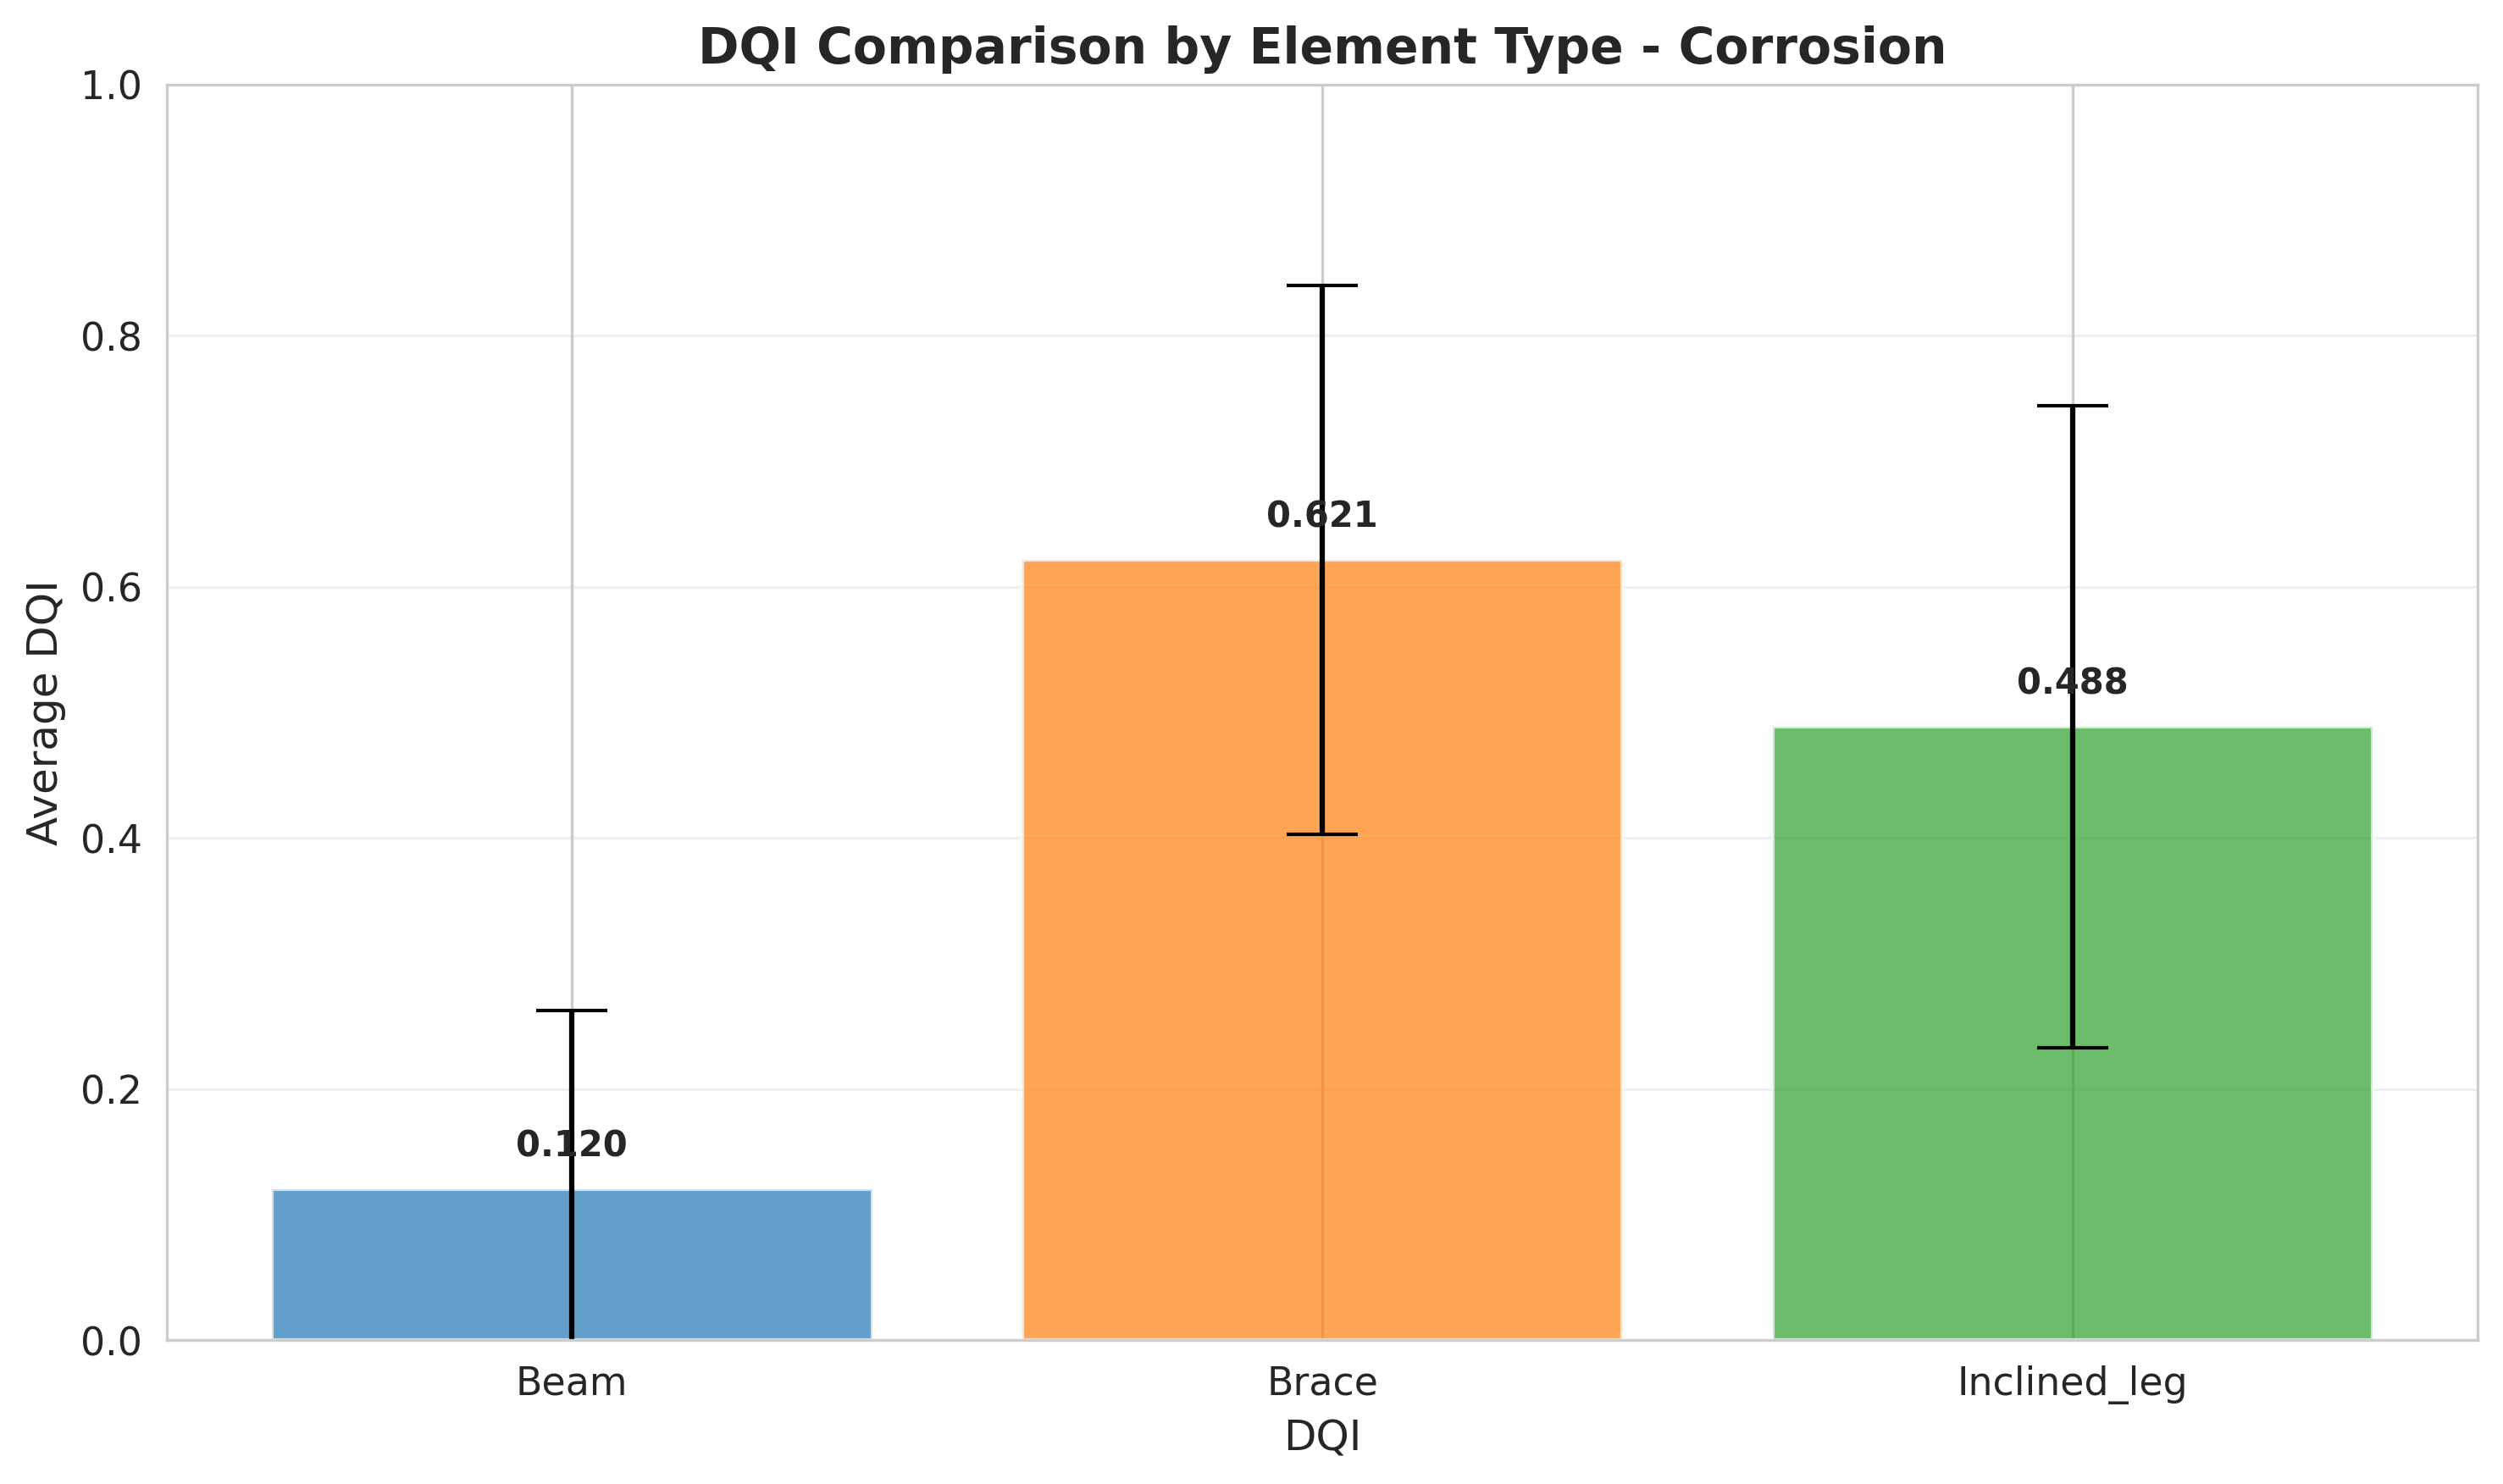
\includegraphics[width=0.9\columnwidth]{../outputs/resultados_nuevos/corrosion_2026/figures/ICD_by_element_type_corrosion.png}
    \caption{DQI sensitivity curves by element type under progressive corrosion scenarios.}
    \label{fig:corrosion_element_type}
\end{figure}

A clear dichotomy is observed in the system response. Secondary elements (braces and inclined members) exhibit a high DQI growth rate, crossing the reliable detection threshold (DQI~$> 0.7$) at damage levels as low as 30\%. This validates the algorithm's capacity to exploit local mode sensitivity in lower-stiffness members.

In contrast, main legs display a nearly flat response curve until cross-sectional loss exceeds 50--60\%. This behaviour is attributed to the high axial and bending stiffness of the legs, which dominates the global structural response; small perturbations in these members are masked by structural redundancy, hampering early identification through frequency or global mode shape changes.

\subsection{Sensitivity to Denting Scenarios}

Figure~\ref{fig:abolladura_element_type} presents the results for impact damage (denting), which produces a drastic but localised reduction of the moment of inertia.

\begin{figure}[!ht]
    \centering
    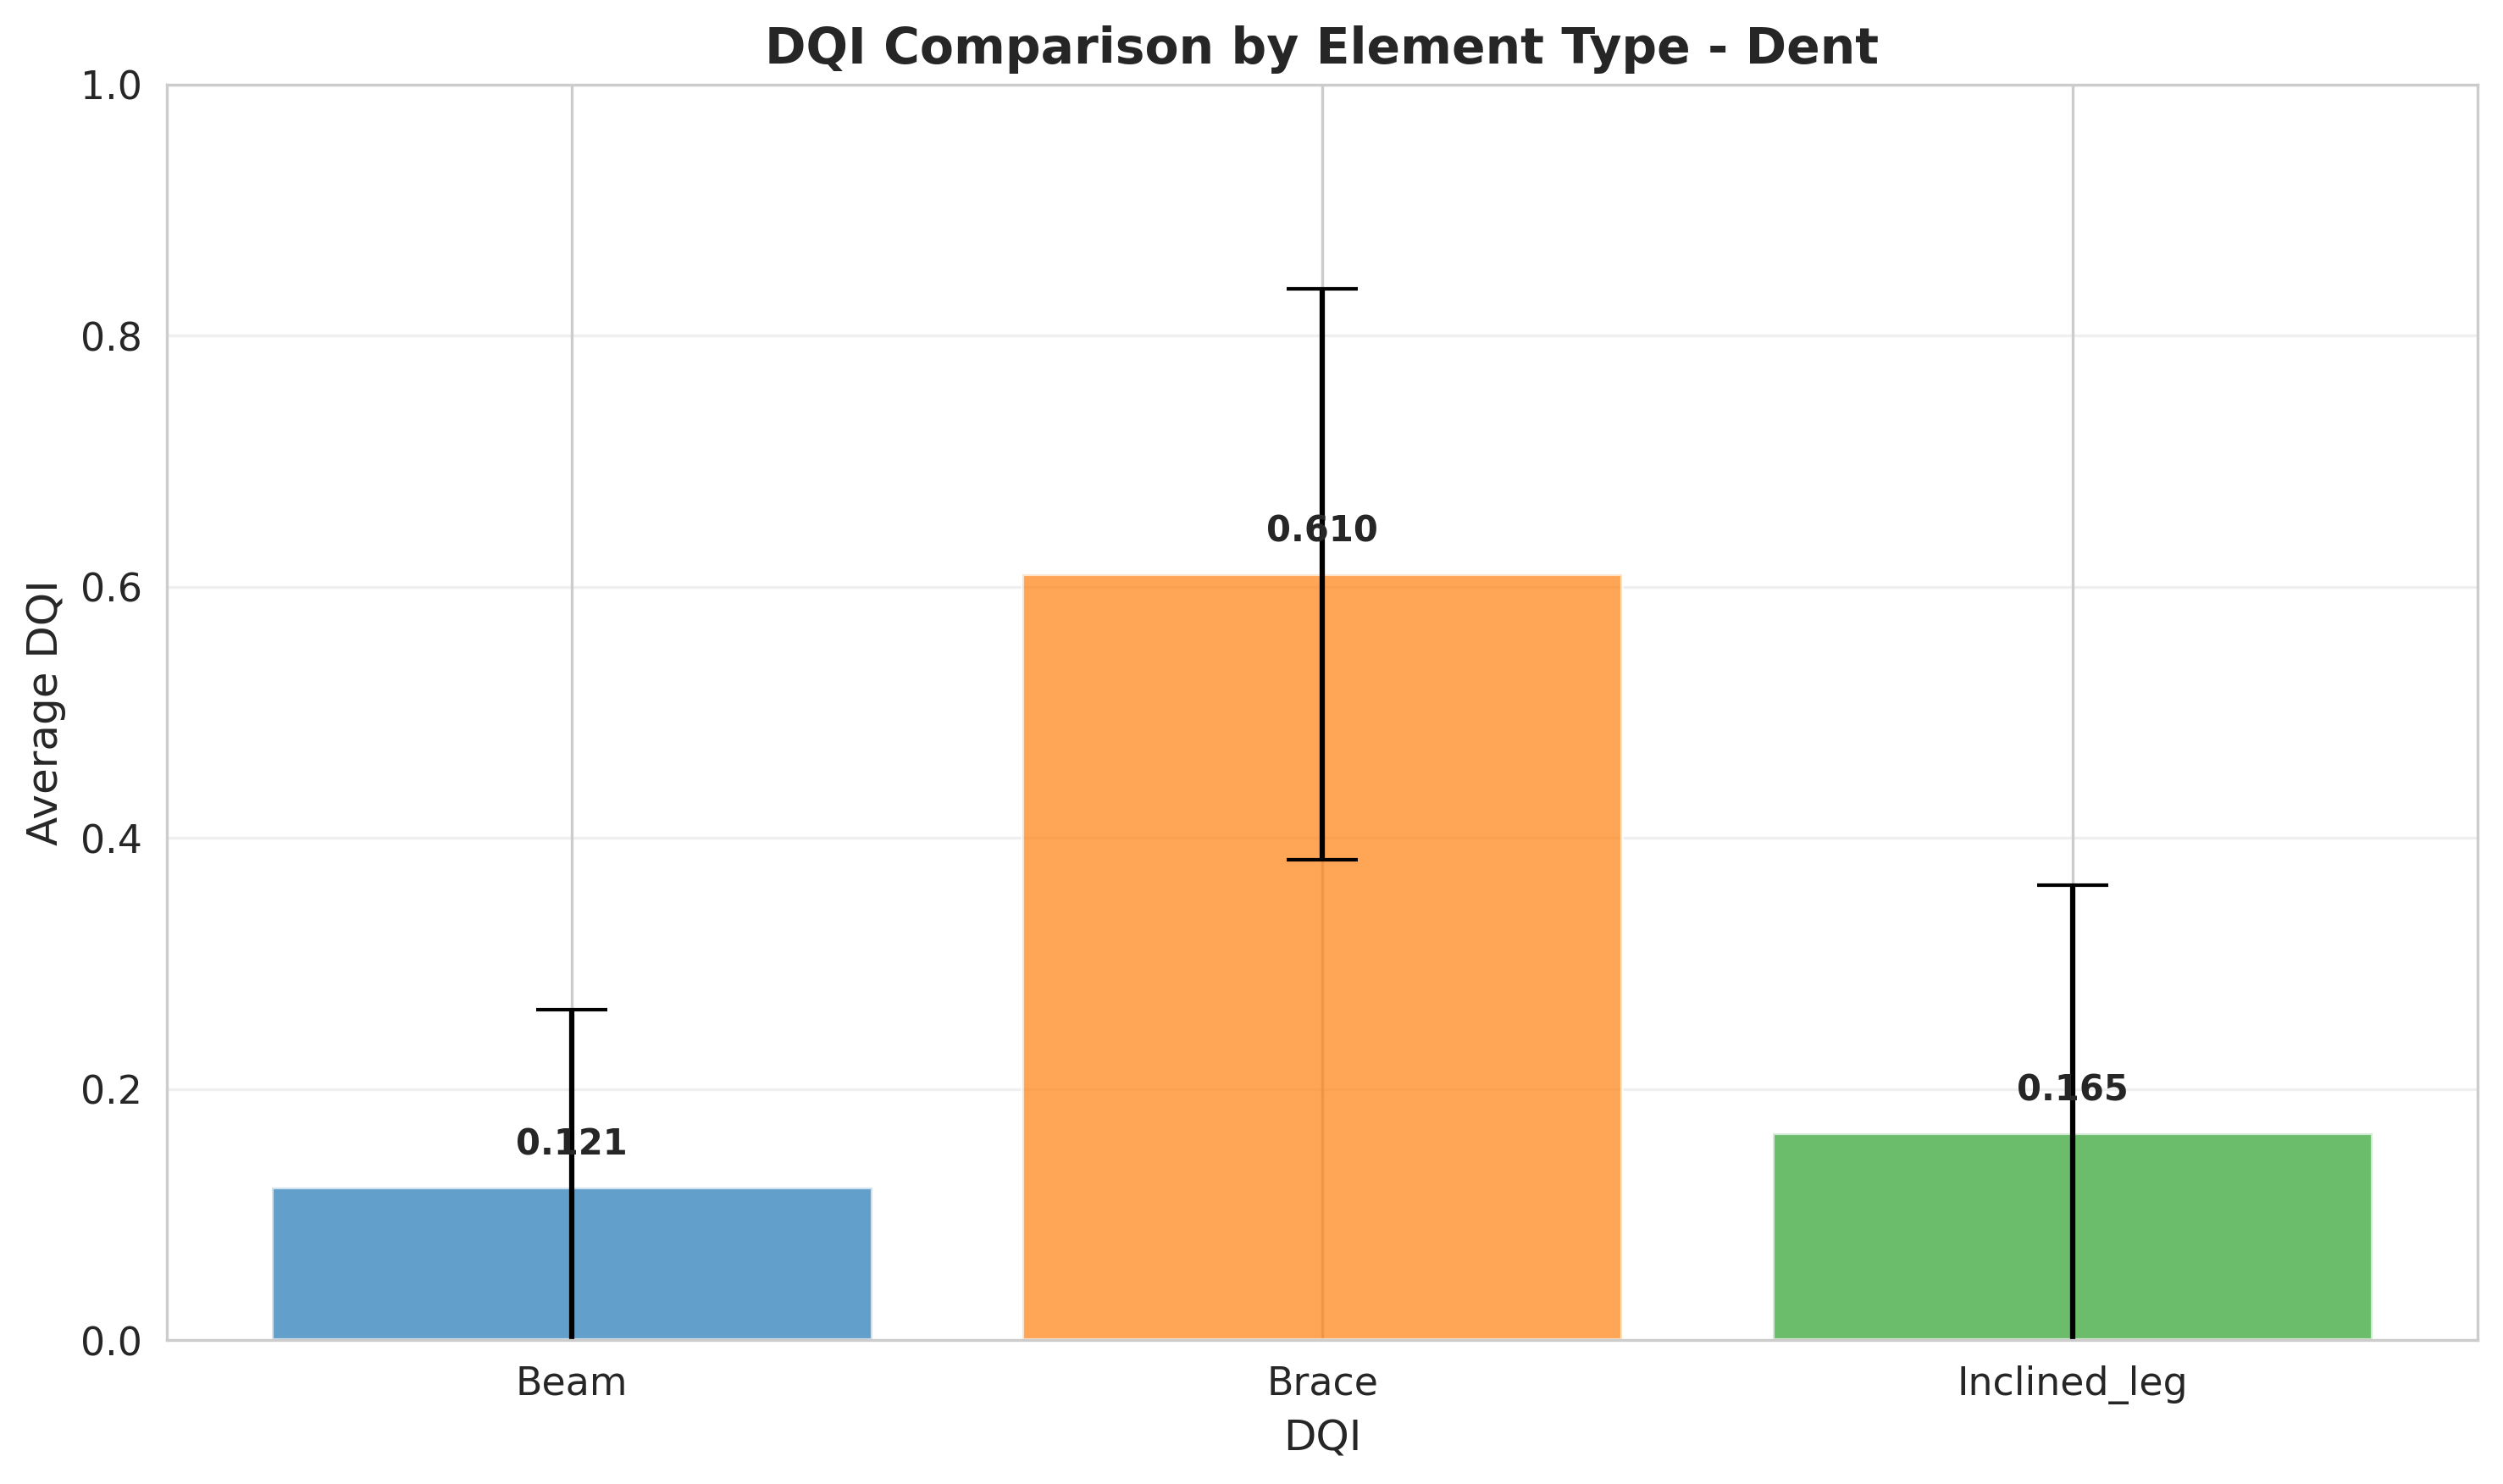
\includegraphics[width=0.9\columnwidth]{../outputs/resultados_nuevos/abolladuras_2026/figures/ICD_by_element_type_abolladura.png}
    \caption{Comparison of DQI sensitivity by element type under denting scenarios.}
    \label{fig:abolladura_element_type}
\end{figure}

Although the physical nature of the damage differs from corrosion, the detectability trend is maintained: diagonal members act as early anomaly indicators. It is noteworthy that, for denting, the detection slope for legs is even more critical, requiring severe deformation before the GA can isolate them. This suggests that, for the monitoring of main legs, the DQI should be supplemented with local inspections in high impact-risk zones.

\subsection{Zone Influence Analysis (Depth)}

To determine whether depth affects diagnostic reliability, the structure was segmented into the five vertical zones defined in Figure~\ref{fig:zonas_plataforma}: the Splash Zone, three intermediate submerged spans (Sub\,1, Sub\,2, and Sub\,3), and the Mudline. Figures~\ref{fig:corrosion_zone} and \ref{fig:abolladura_zone} compare DQI performance across these regions.

\FloatBarrier
\begin{figure*}[!t]
    \centering
    \begin{subfigure}[b]{0.48\textwidth}
        \centering
        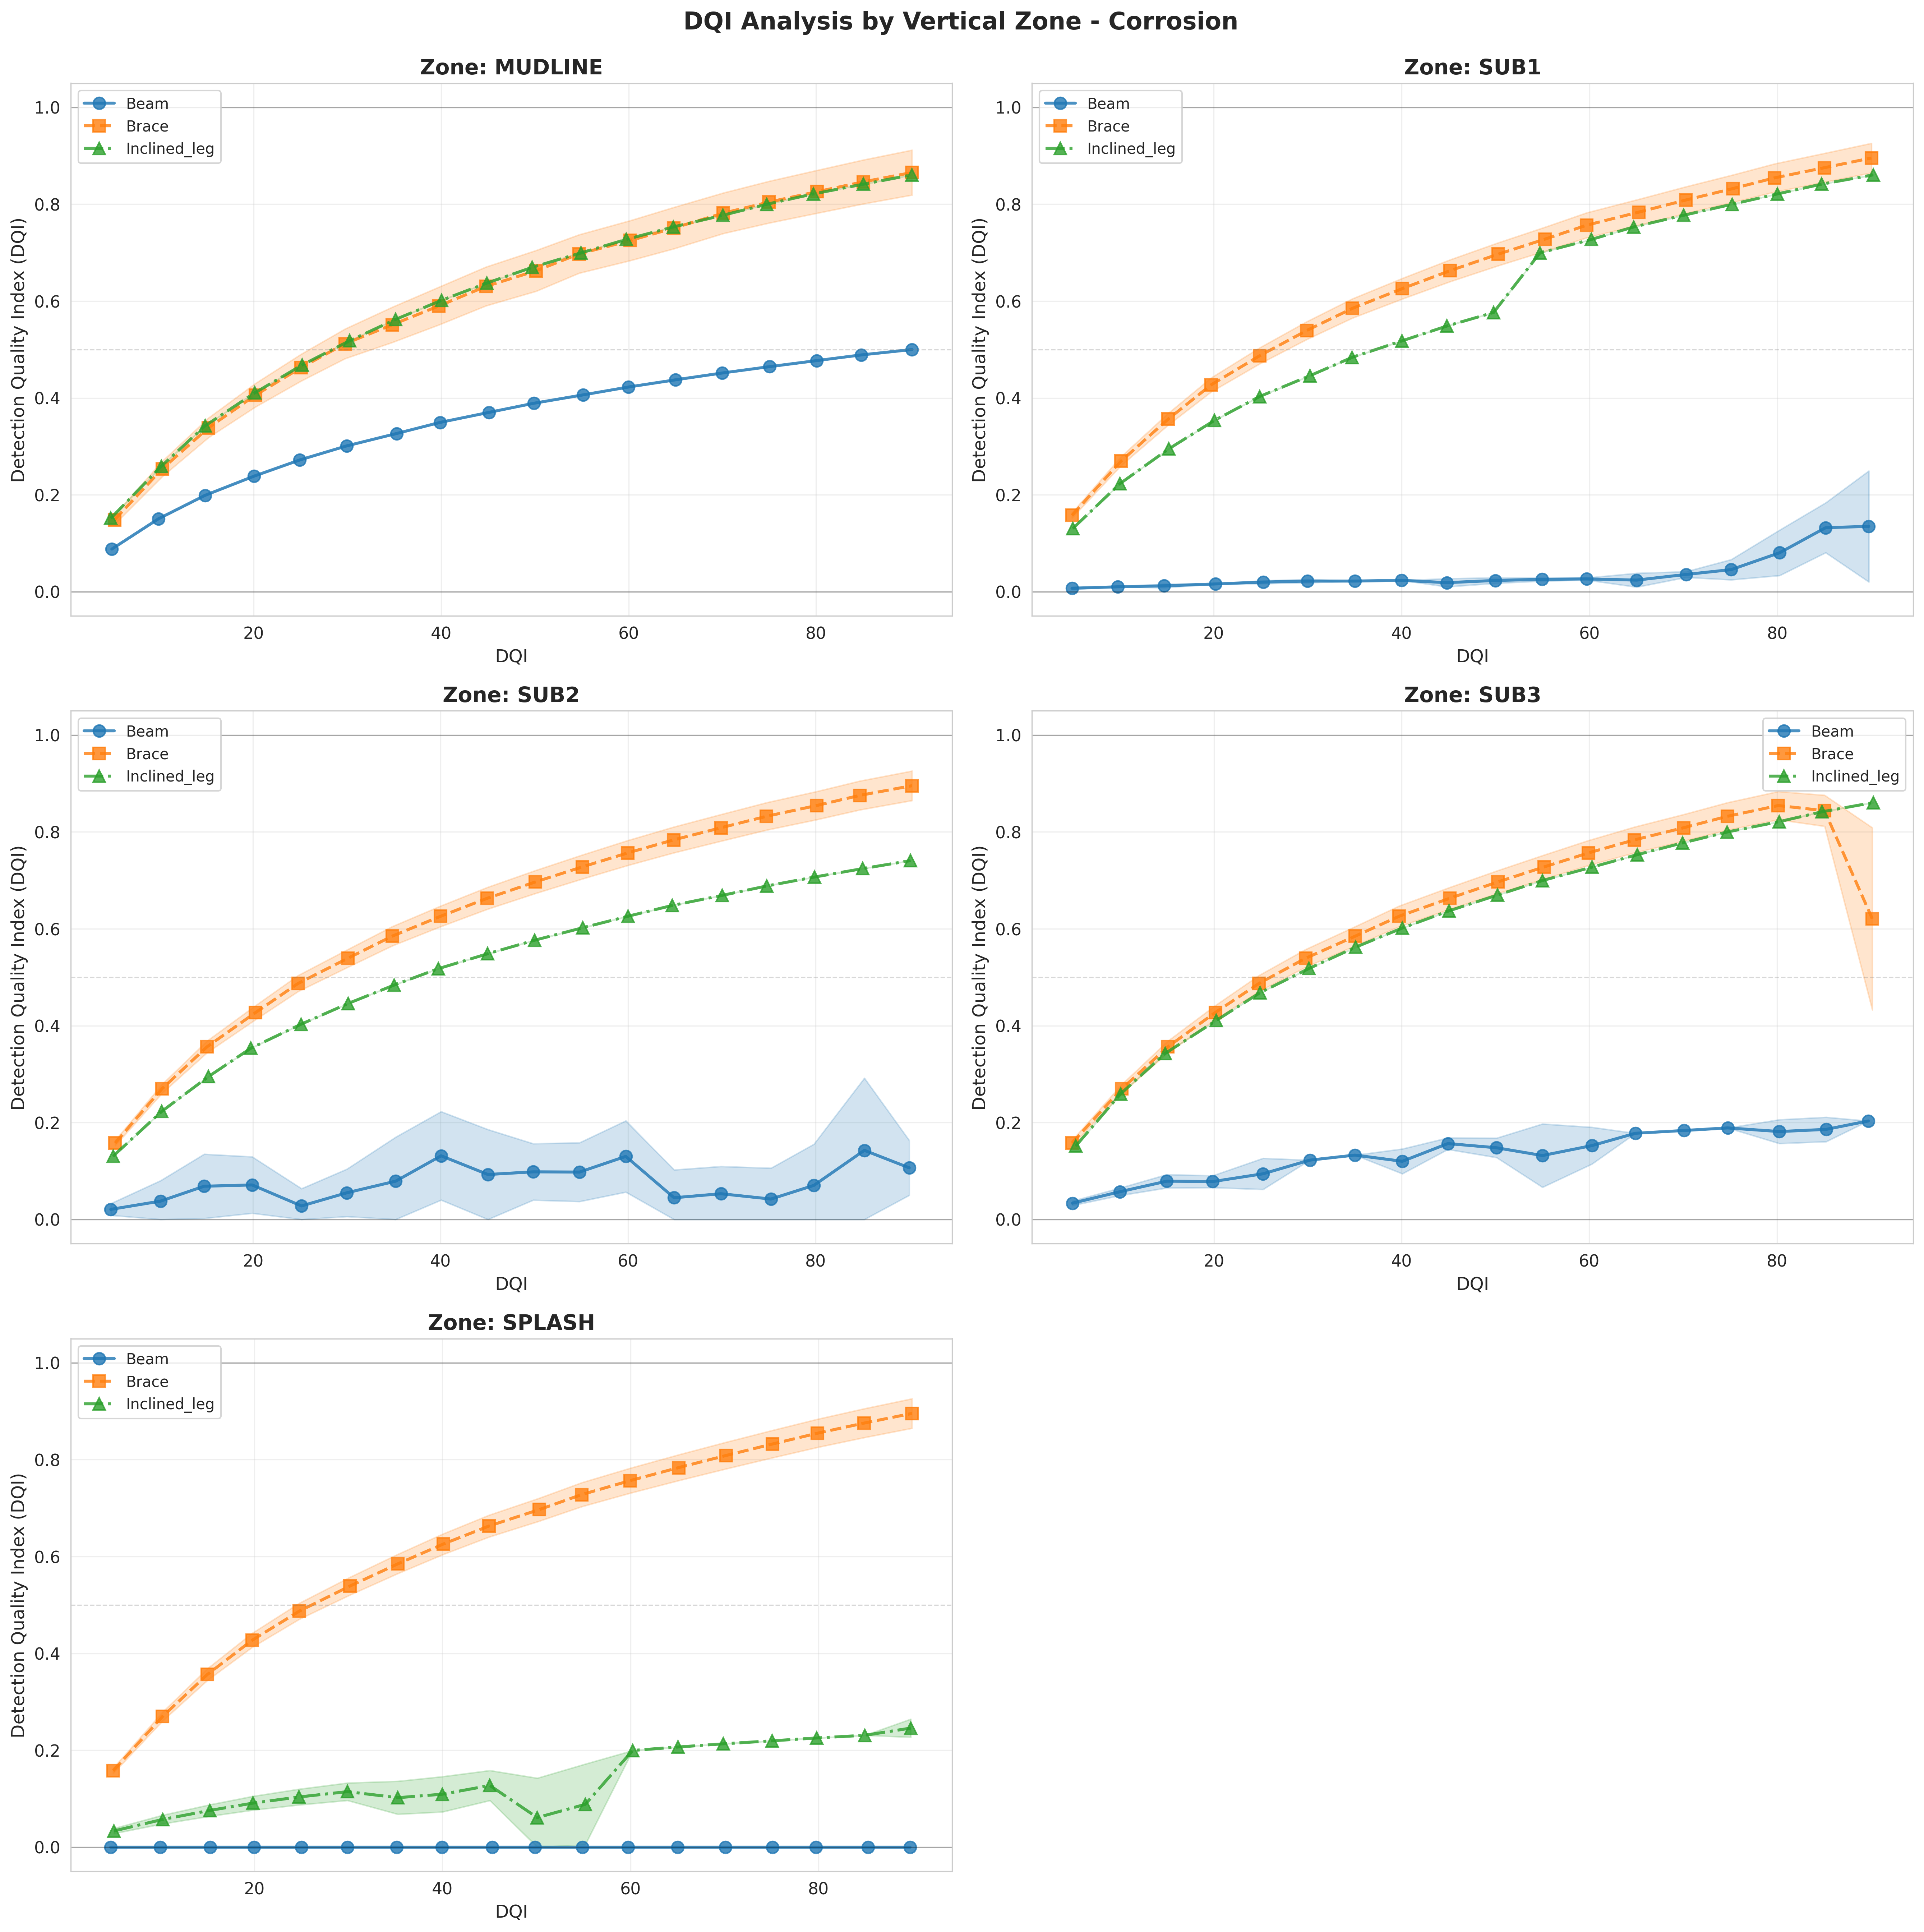
\includegraphics[width=\linewidth]{../outputs/resultados_nuevos/corrosion_2026/figures/ICD_by_zone_corrosion.png}
        \caption{Performance under Corrosion Scenarios.}
        \label{fig:corrosion_zone}
    \end{subfigure}\hfill
    \begin{subfigure}[b]{0.48\textwidth}
        \centering
        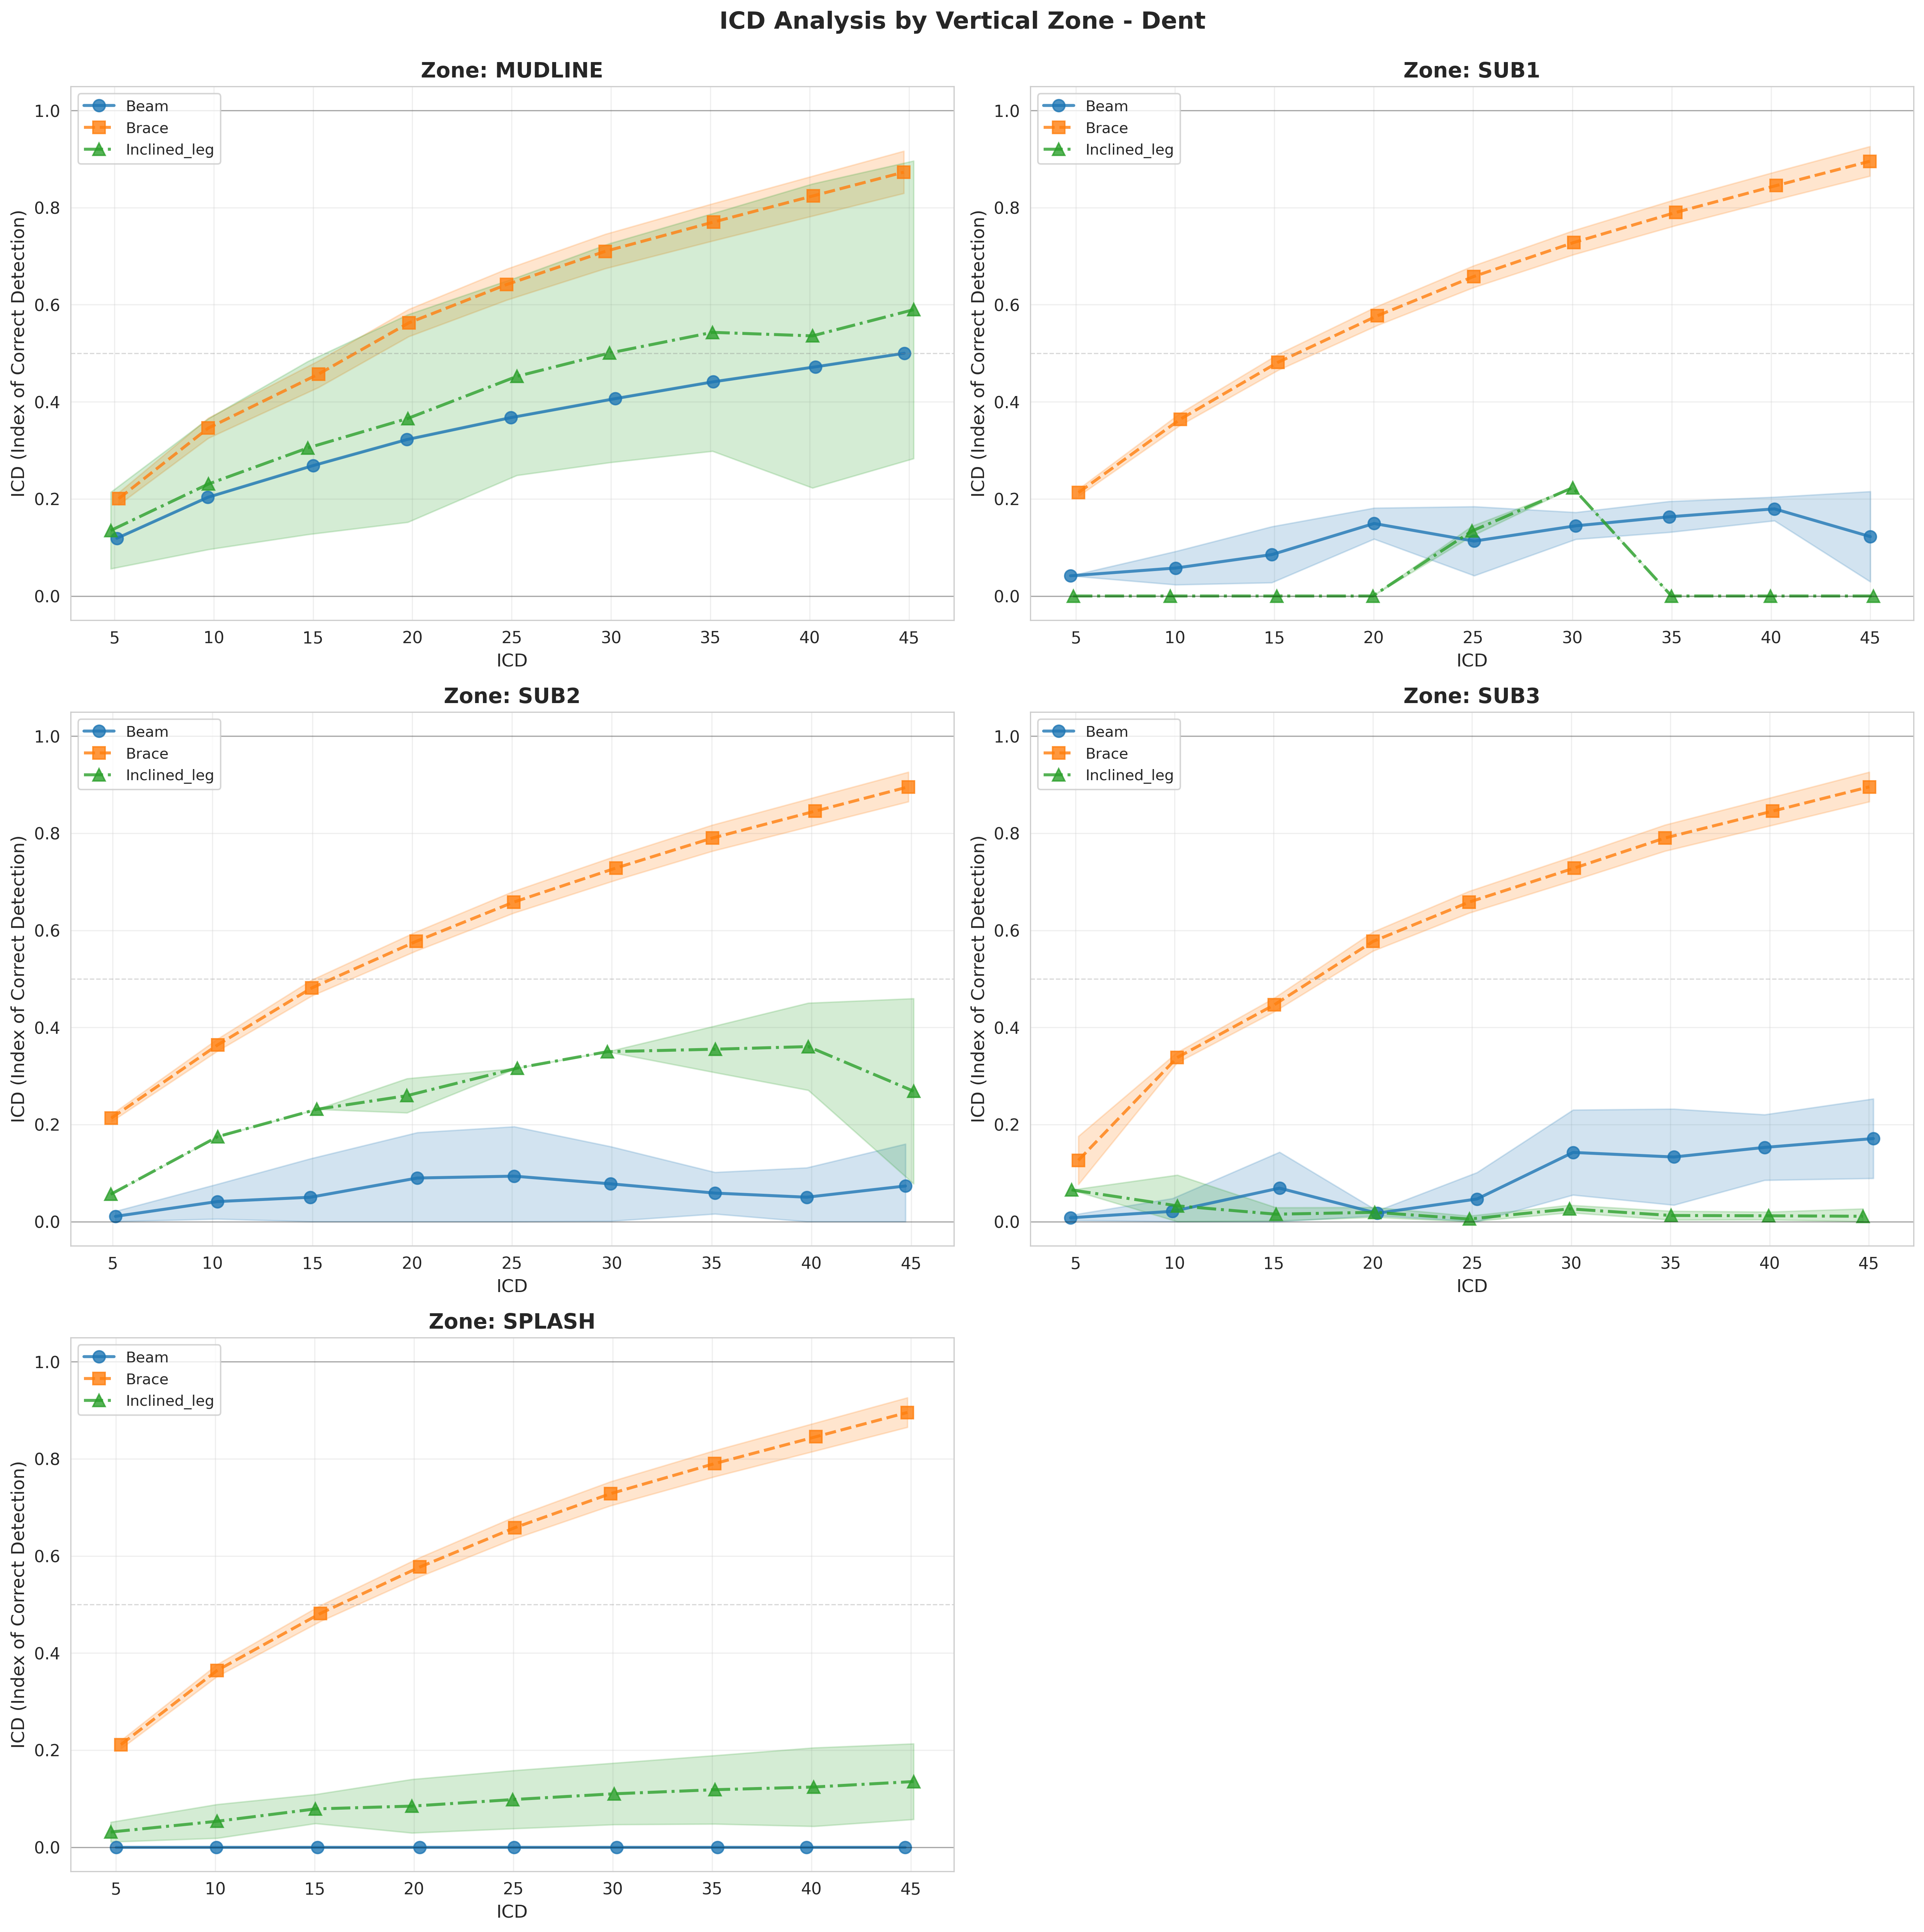
\includegraphics[width=\linewidth]{../outputs/resultados_nuevos/abolladuras_2026/figures/ICD_by_zone_abolladura.png}
        \caption{Performance under Denting Scenarios.}
        \label{fig:abolladura_zone}
    \end{subfigure}
    \caption{Influence of vertical damage location on detection quality (DQI).}
    \label{fig:zone_analysis}
\end{figure*}

\FloatBarrier
\begin{figure}[!ht]
    \centering
    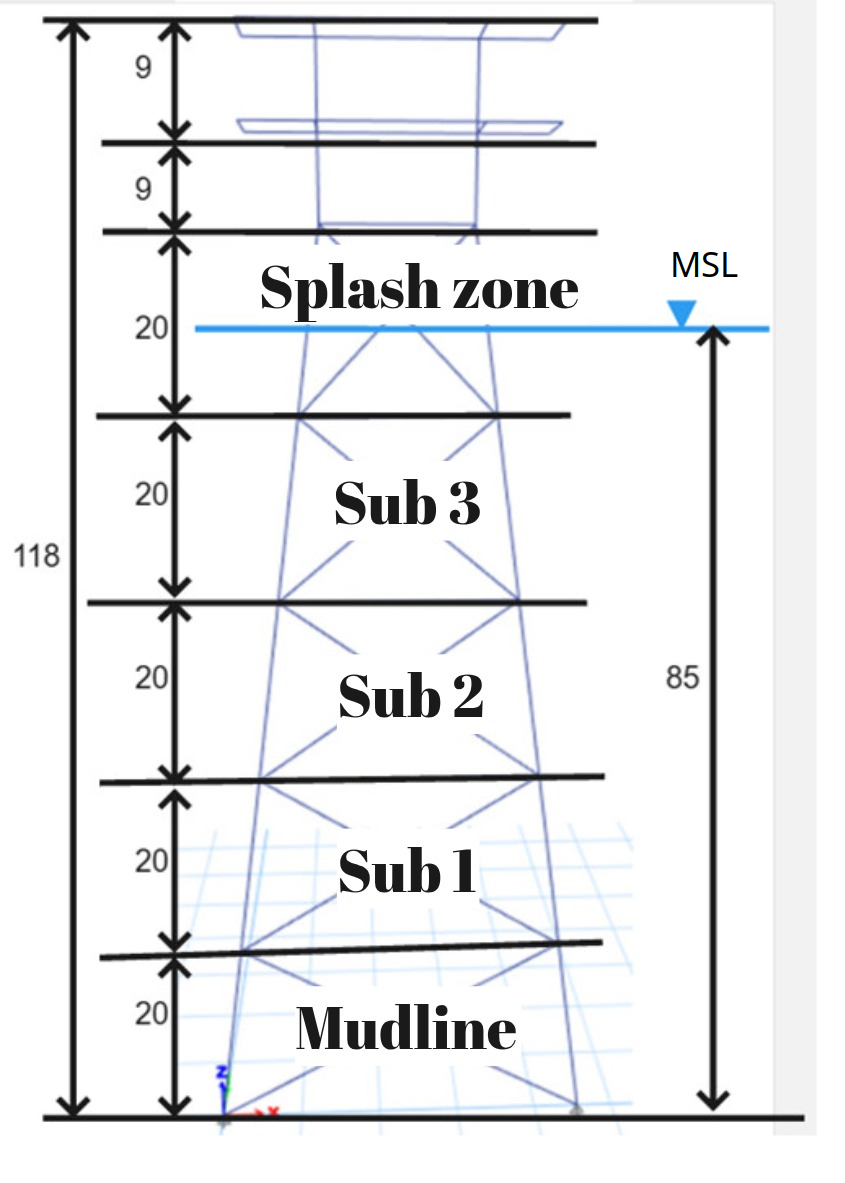
\includegraphics[width=0.55\columnwidth]{figs/008_nombres_zonas_estudio_modelo_plataforma_marina_splashzone_subs_y_mudline_en_una_sola_grafica.png}
    \caption{Vertical zonation of the jacket-type platform: depth-based delineation of the study zones.
             Elevations are expressed in metres referenced to Mean Sea Level (MSL).}
    \label{fig:zonas_plataforma}
\end{figure}

The analysis reveals a slight advantage in the detectability of damage located in the Splash Zone and intermediate submerged spans compared to the Mudline. This is consistent with modal theory: fundamental bending modes display larger displacement and curvature amplitudes at the top of the structure (cantilever behaviour), improving the signal-to-noise ratio for the identification algorithms. Nevertheless, the stiffness hierarchy (Element Type) remains the predominant factor over the spatial location of damage.

% ─────────────────────────────────────────────────────────────────────────────
% §4.4  EXPERIMENTAL DESIGN
% ─────────────────────────────────────────────────────────────────────────────
\subsection{Experimental Design and Case Coverage}
\label{subsec:disenio_experimental}

Statistical validation is supported by a total of 3{,}240 GA runs: 1{,}080 for denting
(120 elements $\times$ 9 severity levels: 5\%--45\%) and 2{,}160 for corrosion
(120 elements $\times$ 18 severity levels: 5\%--90\%). Table~\ref{tab:casos_experimentales}
summarises the distribution of runs by damage type and element type.

\begin{table*}[!ht]
  \centering
  \caption{Summary of the numerical experiment: damage scenarios evaluated with the DQI+GA framework.}
  \label{tab:casos_experimentales}
  \begin{tabular}{lrrrrr}
    \toprule
    Damage Type & N Elements & Severity Range [\%] & Step [\%] & Levels & Total Runs \\
    \midrule
    Denting & 120 & 5--45 & 5 & 9 & 1,080 \\
    Corrosion & 120 & 5--90 & 5 & 18 & 2,160 \\
    \midrule
    \textbf{Total} & & & & & \textbf{3,240} \\
    \bottomrule
  \end{tabular}
\end{table*}

Figure~\ref{fig:distribucion_experimental} summarises the experimental design from three
complementary perspectives. Panel~(a) confirms the intentional asymmetry in the number of
runs: 2{,}160 for corrosion versus 1{,}080 for denting, a difference that reflects the
wider severity range explored (18 vs.\ 9 damage levels). Panel~(b) shows that brace elements
(X-diagonals) constitute \textbf{67\%} of the total 120 structural members (80 elements), a
proportion that confers greater statistical representativeness to the results for this element
type---precisely those showing the best detection performance in the subsequent analysis.
Panel~(c) confirms that each vertical level of the model contains an equivalent typological
composition, ensuring inter-zone comparability.

\begin{figure*}[!t]
    \centering
    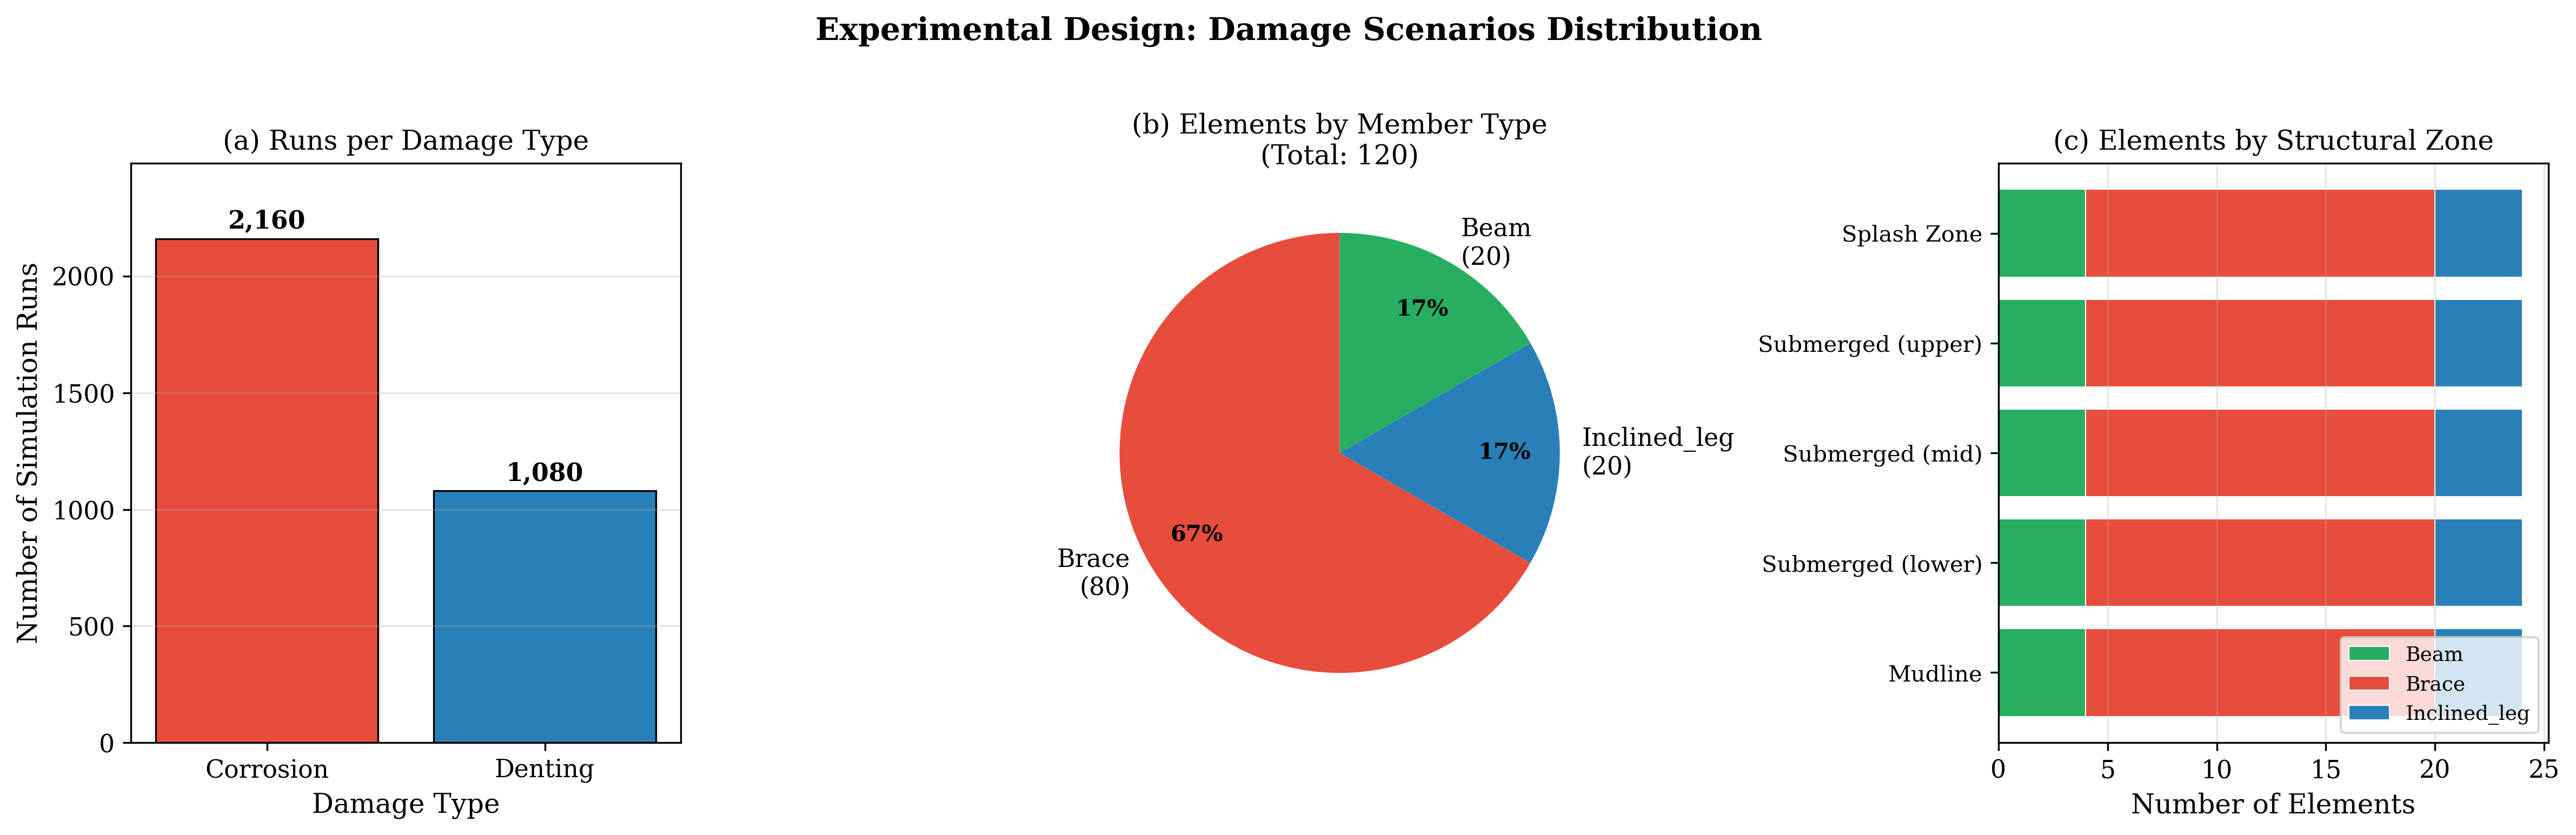
\includegraphics[width=0.9\textwidth]{../outputs/resultados_nuevos/experimental_design_distribution.png}
    \caption{Experimental design: (a)~simulation runs by damage type (Corrosion:
             2{,}160; Denting: 1{,}080); (b)~typological composition of the 120 model
             elements (\textit{Braces}: 67\%, \textit{Beams}: 17\%,
             \textit{Inclined legs}: 17\%); (c)~element distribution by vertical structural zone.}
    \label{fig:distribucion_experimental}
\end{figure*}

The platform is divided into five vertical levels (see Figure~\ref{fig:zonas_plataforma}): the Mudline (base) and three intermediate submerged spans (Sub\,1, Sub\,2, and Sub\,3) of 20~m each, plus the Splash Zone at the air--water interface, resulting in a total submerged draft of 85~m referenced to Mean Sea Level.

% ─────────────────────────────────────────────────────────────────────────────
% §4.5  CLASSIFICATION METRICS
% ─────────────────────────────────────────────────────────────────────────────
\subsection{Classification Metrics: Precision and Recall}
\label{subsec:metricas_clasificacion}

To quantify system performance beyond the DQI, standard binary classification metrics are
employed, grounded in the \textbf{confusion matrix} of the problem.
In each GA run, the algorithm produces a prediction vector
$\hat{\mathbf{d}} \in \{0,1\}^{N_\text{el}}$ ($1$~=~element predicted as damaged)
compared against the ground-truth label $\mathbf{d}^* \in \{0,1\}^{N_\text{el}}$
(exactly one damaged element per run). Four outcomes arise from this comparison:
\textit{True Positive} (TP: damaged element correctly identified),
\textit{False Positive} (FP: healthy element flagged as damaged),
\textit{False Negative} (FN: damaged element not detected), and
\textit{True Negative} (TN: healthy element correctly discarded).
The two principal derived metrics are:

\begin{align}
    \text{Precision} &= \frac{TP}{TP + FP} \label{eq:precision} \\[4pt]
    \text{Recall}    &= \frac{TP}{TP + FN} \label{eq:recall}
\end{align}

\noindent In the structural integrity context, Precision quantifies how many of the elements flagged as damaged are truly damaged (false inspection alarm cost); Recall quantifies how many truly damaged elements are detected (missed-damage cost).
Table~\ref{tab:metricas_compacta} reports the mean values by element type and damage scenario.

% Table follows below, before Topology-Weighted Precision subsection.

Table~\ref{tab:metricas_compacta} shows that Recall values are consistently high (close to 1.0),
confirming the DQI's capacity to detect the damaged element. However, Precision values are
systematically low---particularly for Beams (0.08--0.12)---as a consequence of an inherent
limitation of the classical metric: it penalises all False Positives (FPs) identically,
irrespective of their topological distance to the damaged element. In the jacket lattice
network, an adjacent FP ($d=1$) reflects stress redistribution in the immediate vicinity and
carries a radically different engineering meaning from one at the far end of the structure
($d=9$, the topological diameter of this platform's connectivity graph). This uniform penalisation systematically underestimates the true localisation quality
of the algorithm and reduces the statistical value of Precision as a diagnostic reliability
indicator in lattice platforms. Section~\ref{subsec:precision_ponderada} introduces the
\textbf{Topology-Weighted Precision} ($\text{Precision}_w$), which corrects this deficiency
by assigning weights proportional to the topological distance of each FP, providing a more
robust assessment of localiser performance.

A distinct behaviour, evident in Table~\ref{tab:metricas_compacta}, deserves explicit
discussion: horizontal beams exhibit high Recall (close to $1.0$, the anomaly is detected)
yet the localisation is never assigned to the beam itself but consistently to an adjacent
member ($D=0.5$ in all beam cases, which is why the AUC-ROC is reported as N/A for this
member type in Table~\ref{tab:snr_robustness}). This is not a numerical artefact---the
sensitivity analysis of Section~\ref{sec:metodologia} confirms that beams remain
unlocalisable across the full range of $\beta$---but a direct consequence of modal
mechanics. The detectability of damage in an element through vibration-based indicators is
proportional to the fraction of modal strain energy (MSE) that the element stores in the
measured modes, since the sensitivity of the $i$-th natural frequency to a stiffness loss
in element $e$ scales with $\text{MSE}_{i,e}=\tfrac{1}{2}\,\boldsymbol{\phi}_i^{\!\top}\mathbf{k}_e\,\boldsymbol{\phi}_i$
\citep{doebling1996damage}. In a cantilever-type jacket, the low-order modes ($N_m=6$) are
dominated by global lateral bending and torsion: the diagonal braces and inclined legs
resist the lateral shear through truss action and therefore accumulate high axial strain
energy, whereas the horizontal beams---oriented transversely to the dominant bending
direction and connecting nodes that move almost in phase within each horizontal plane---store
comparatively negligible MSE in these modes. A stiffness reduction in a beam thus produces an
almost imperceptible change in the global modal and flexibility signatures, and the residual
signal at its end nodes is dominated by the high-MSE braces concurring at the same joints. The
GA, maximising the detection signal, consequently attributes the anomaly to the adjacent brace
($d=1$), yielding indirect localisation rather than failure. This mechanism explains the
otherwise paradoxical combination of high Recall and failed localisation for beams, and
implies that reliable beam monitoring would require either higher-order modes---where their
local MSE becomes appreciable---or complementary local instrumentation.

% ─────────────────────────────────────────────────────────────────────────────
% §4.6  TOPOLOGY-WEIGHTED PRECISION  [NOVEL CONTRIBUTION]
% ─────────────────────────────────────────────────────────────────────────────
\begin{table*}[!ht]
    \centering
    \caption{Summary of classification performance at key severity levels. The low Precision values reflect a structural limitation of the classical metric, which assigns equal penalty to all false positives regardless of their topological distance to the damaged element (see Section~\ref{subsec:precision_ponderada}).}
    \label{tab:metricas_compacta}
    \begin{tabular}{llrrr}
        \toprule
        Damage Type & Element & Severity & Precision & Recall \\
        \midrule
        Denting & Brace & 10\% & 0.404 & 0.952 \\
        Denting & Brace & 20\% & 0.398 & 0.952 \\
        Denting & Brace & 30\% & 0.365 & 0.952 \\
        Denting & Brace & 45\% & 0.370 & 0.952 \\
        \cmidrule{2-5}
        Denting & Inclined Leg & 10\% & 0.152 & 0.600 \\
        Denting & Inclined Leg & 20\% & 0.093 & 0.750 \\
        Denting & Inclined Leg & 30\% & 0.122 & 1.000 \\
        Denting & Inclined Leg & 45\% & 0.078 & 0.700 \\
        \cmidrule{2-5}
        Denting & Beam & 10\% & 0.084 & 1.000 \\
        Denting & Beam & 20\% & 0.094 & 1.000 \\
        Denting & Beam & 30\% & 0.116 & 1.000 \\
        Denting & Beam & 45\% & 0.098 & 1.000 \\
        \midrule
        Corrosion & Brace & 20\% & 0.381 & 0.952 \\
        Corrosion & Brace & 40\% & 0.377 & 0.952 \\
        Corrosion & Brace & 60\% & 0.381 & 0.952 \\
        Corrosion & Brace & 90\% & 0.319 & 0.905 \\
        \cmidrule{2-5}
        Corrosion & Inclined Leg & 20\% & 0.286 & 1.000 \\
        Corrosion & Inclined Leg & 40\% & 0.263 & 1.000 \\
        Corrosion & Inclined Leg & 60\% & 0.333 & 1.000 \\
        Corrosion & Inclined Leg & 90\% & 0.339 & 1.000 \\
        \cmidrule{2-5}
        Corrosion & Beam & 20\% & 0.099 & 1.000 \\
        Corrosion & Beam & 40\% & 0.105 & 1.000 \\
        Corrosion & Beam & 60\% & 0.105 & 1.000 \\
        Corrosion & Beam & 90\% & 0.121 & 1.000 \\
        \bottomrule
    \end{tabular}
\end{table*}

\subsection{Topology-Weighted Precision}
\label{subsec:precision_ponderada}

\subsubsection{Limitation of Classical Precision}

Classical Precision treats all False Positives (FPs) with equal penalisation,
regardless of their spatial proximity to the truly damaged element:

\begin{equation}
    \label{eq:precision_clasica}
    \text{Precision} = \frac{TP}{TP + FP}
\end{equation}

This formulation is inadequate in lattice systems where an FP node adjacent
to the damaged element (topological distance $d=1$) carries a very different engineering
interpretation from one located at the opposite end of the structure ($d = 9$).

\subsubsection{Topology-Weighted Precision Formulation}

A novel metric is proposed that assigns a weight $w(d) \in [0, 1)$ to each FP as a function
of its topological distance $d$ to the damaged element, measured in number of structural
members via breadth-first search (BFS) on the connectivity graph:

\begin{equation}
    \label{eq:weight_fn}
    w(d) = \frac{d}{d + 1}
\end{equation}

so that adjacent nodes ($d=1$) receive only 50\% of the penalisation, while
distant nodes ($d \to \infty$) approach the full penalty. The \textbf{Topology-Weighted
Precision} is then:

\begin{equation}
    \label{eq:precision_ponderada}
    \text{Precision}_w = \frac{TP}{TP + \displaystyle\sum_{i \in FP} w(d_i)}
\end{equation}

\subsubsection{FP Distance Distribution}

Figure~\ref{fig:FP_distancias} reveals that approximately 40\% of all FP nodes
are directly adjacent to the damaged element ($d = 1$), with a mean distance of
$\bar{d} \approx 2.2$ members. This finding justifies the need for the topological
correction: classical Precision systematically underestimates the localisation quality
of the GA.

\FloatBarrier
\clearpage

\begin{figure*}[t!]
    \centering
    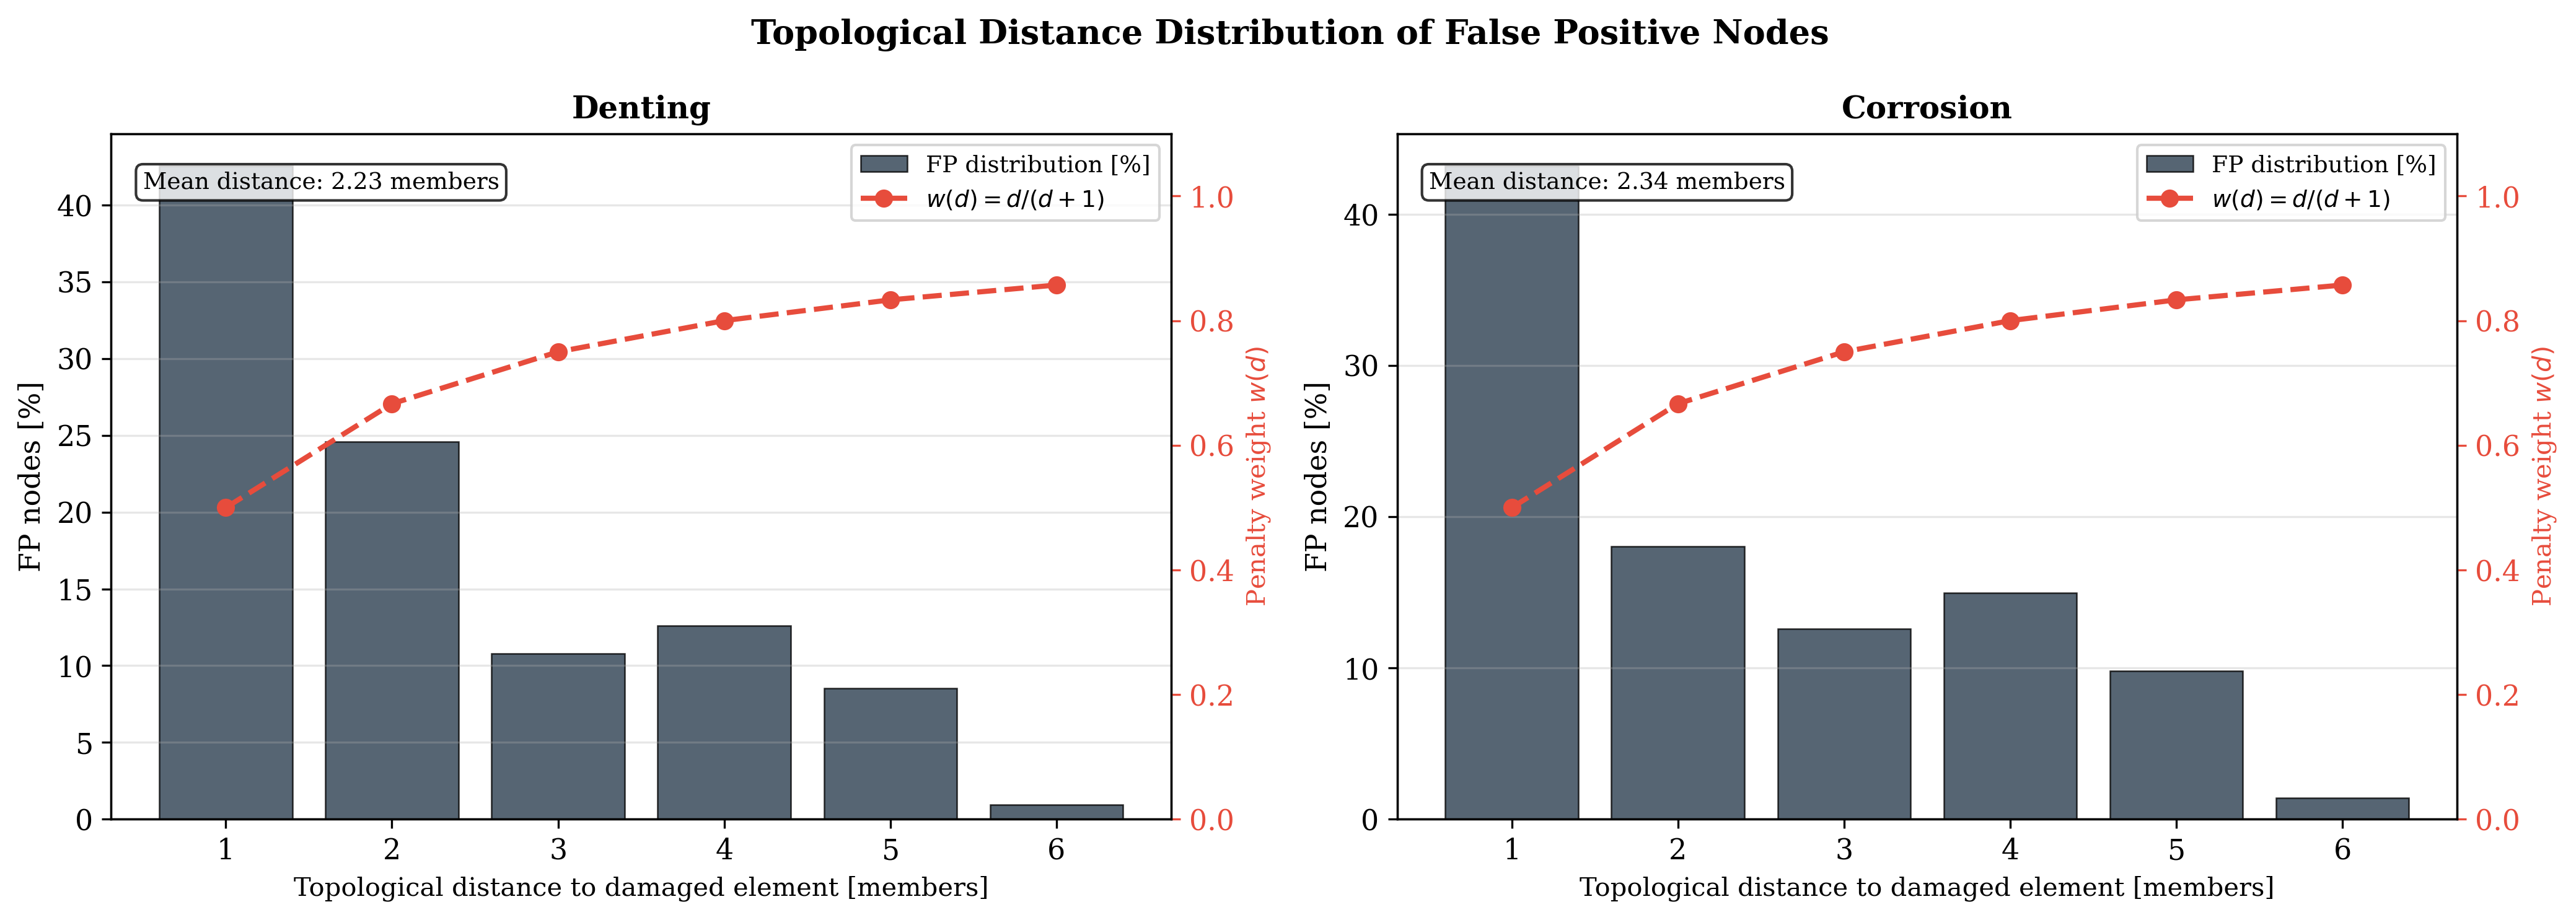
\includegraphics[width=0.9\textwidth]{../outputs/resultados_nuevos/FP_distancia_topologica_distribucion.png}
    \caption{Topological distance distribution of FP nodes to the damaged element for
             Denting (left) and Corrosion (right). The red curve shows the weight function
             $w(d) = d/(d+1)$.}
    \label{fig:FP_distancias}
\end{figure*}

\subsubsection{Quantitative Comparison}

Figure~\ref{fig:precision_global} quantifies the Precision improvement for each element type
when transitioning from the classical to the weighted metric. Braces show the greatest gain
($\Delta \approx +22$ percentage points) in both denting and corrosion scenarios, confirming
that their FP signal is structurally coherent with the localised damage.
Figure~\ref{fig:precision_vs_severidad} details the evolution of classical and weighted
Precision as a function of damage severity.

% The two visualisations are presented separately to avoid joint rendering issues.

\begin{figure*}[!t]
    \centering
    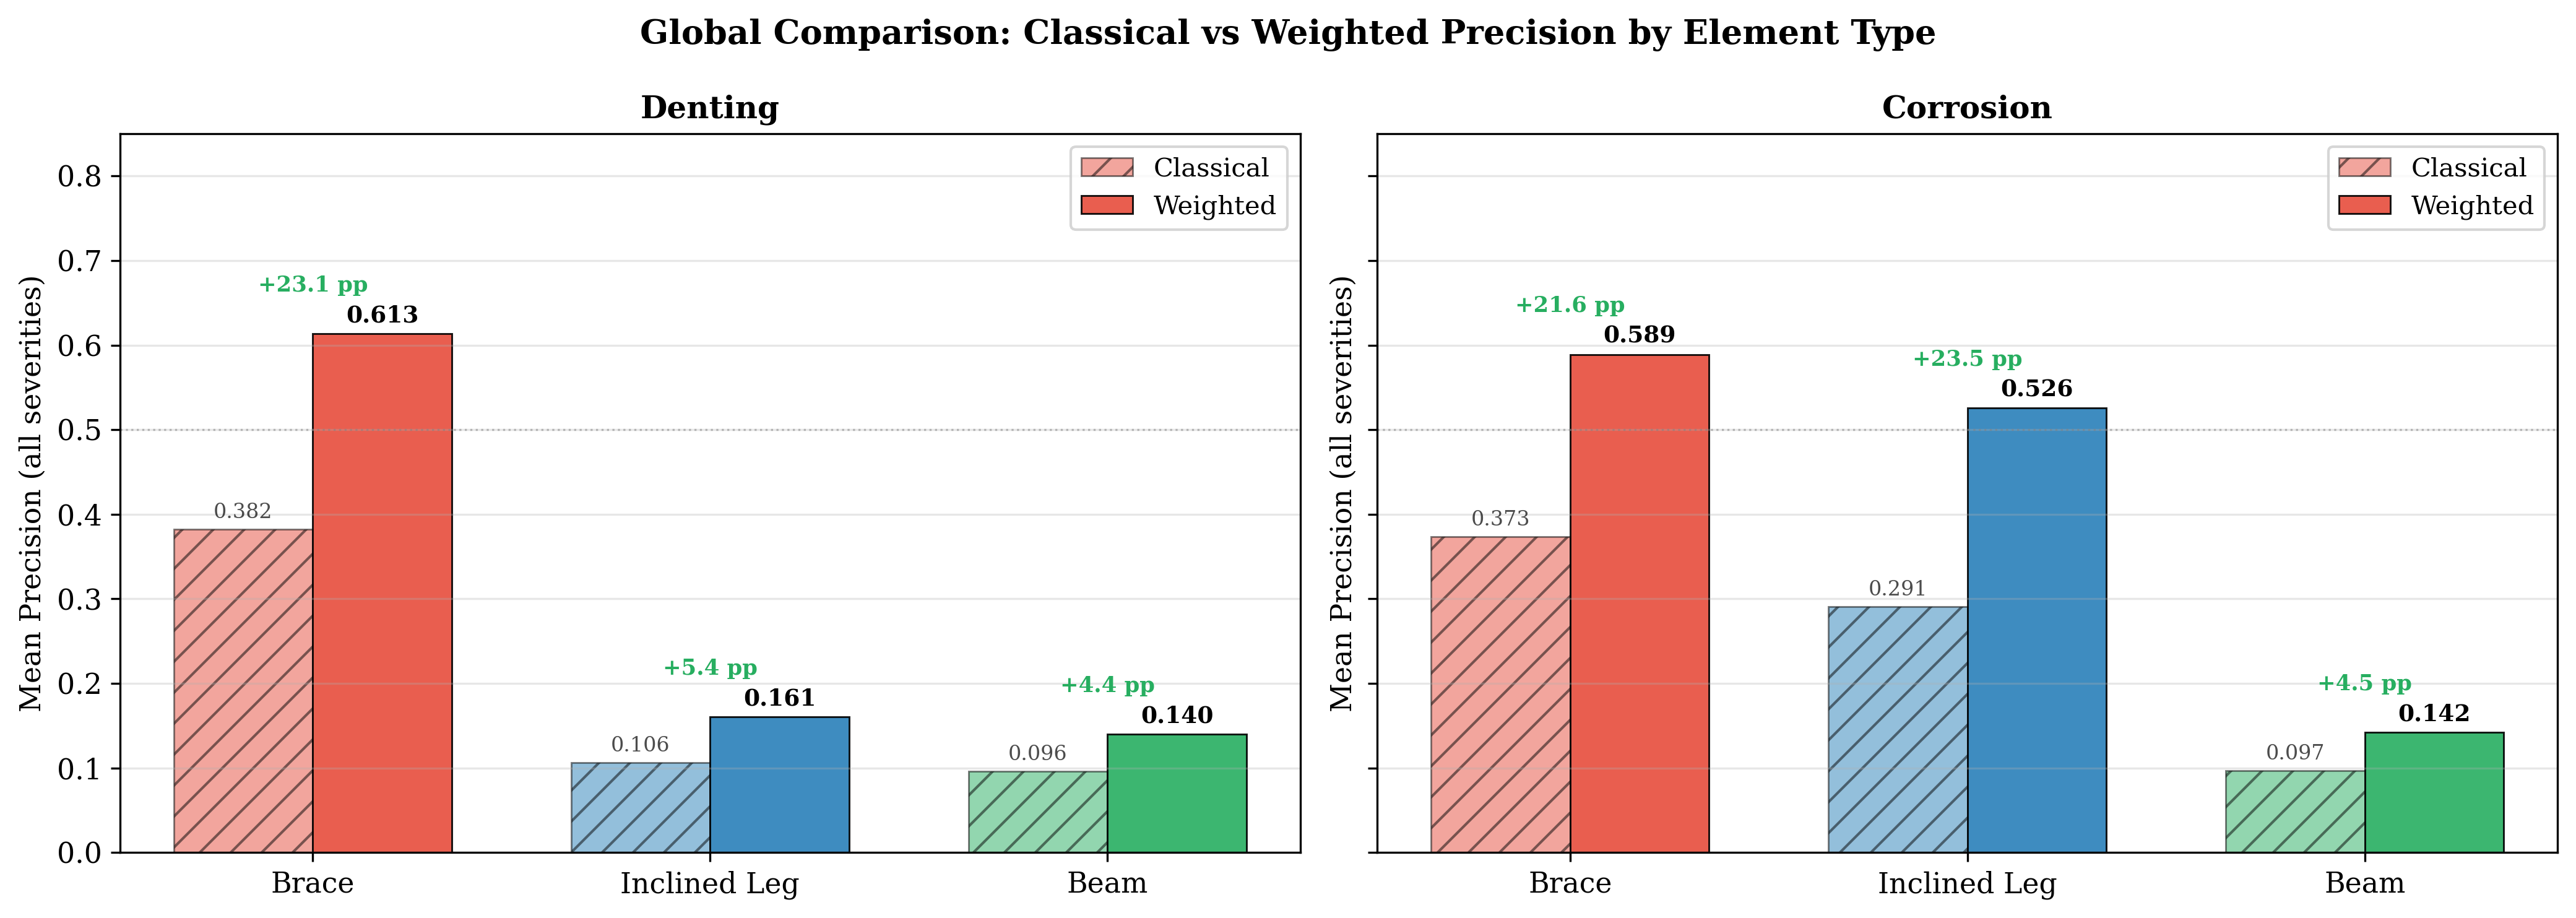
\includegraphics[width=0.9\textwidth]{../outputs/resultados_nuevos/Precision_global_clasica_vs_ponderada.png}
    \caption{Global comparison of Classical vs.\ Topology-Weighted Precision by element type.}
    \label{fig:precision_global}
\end{figure*}

\clearpage

\begin{figure*}[t!]
    \centering
    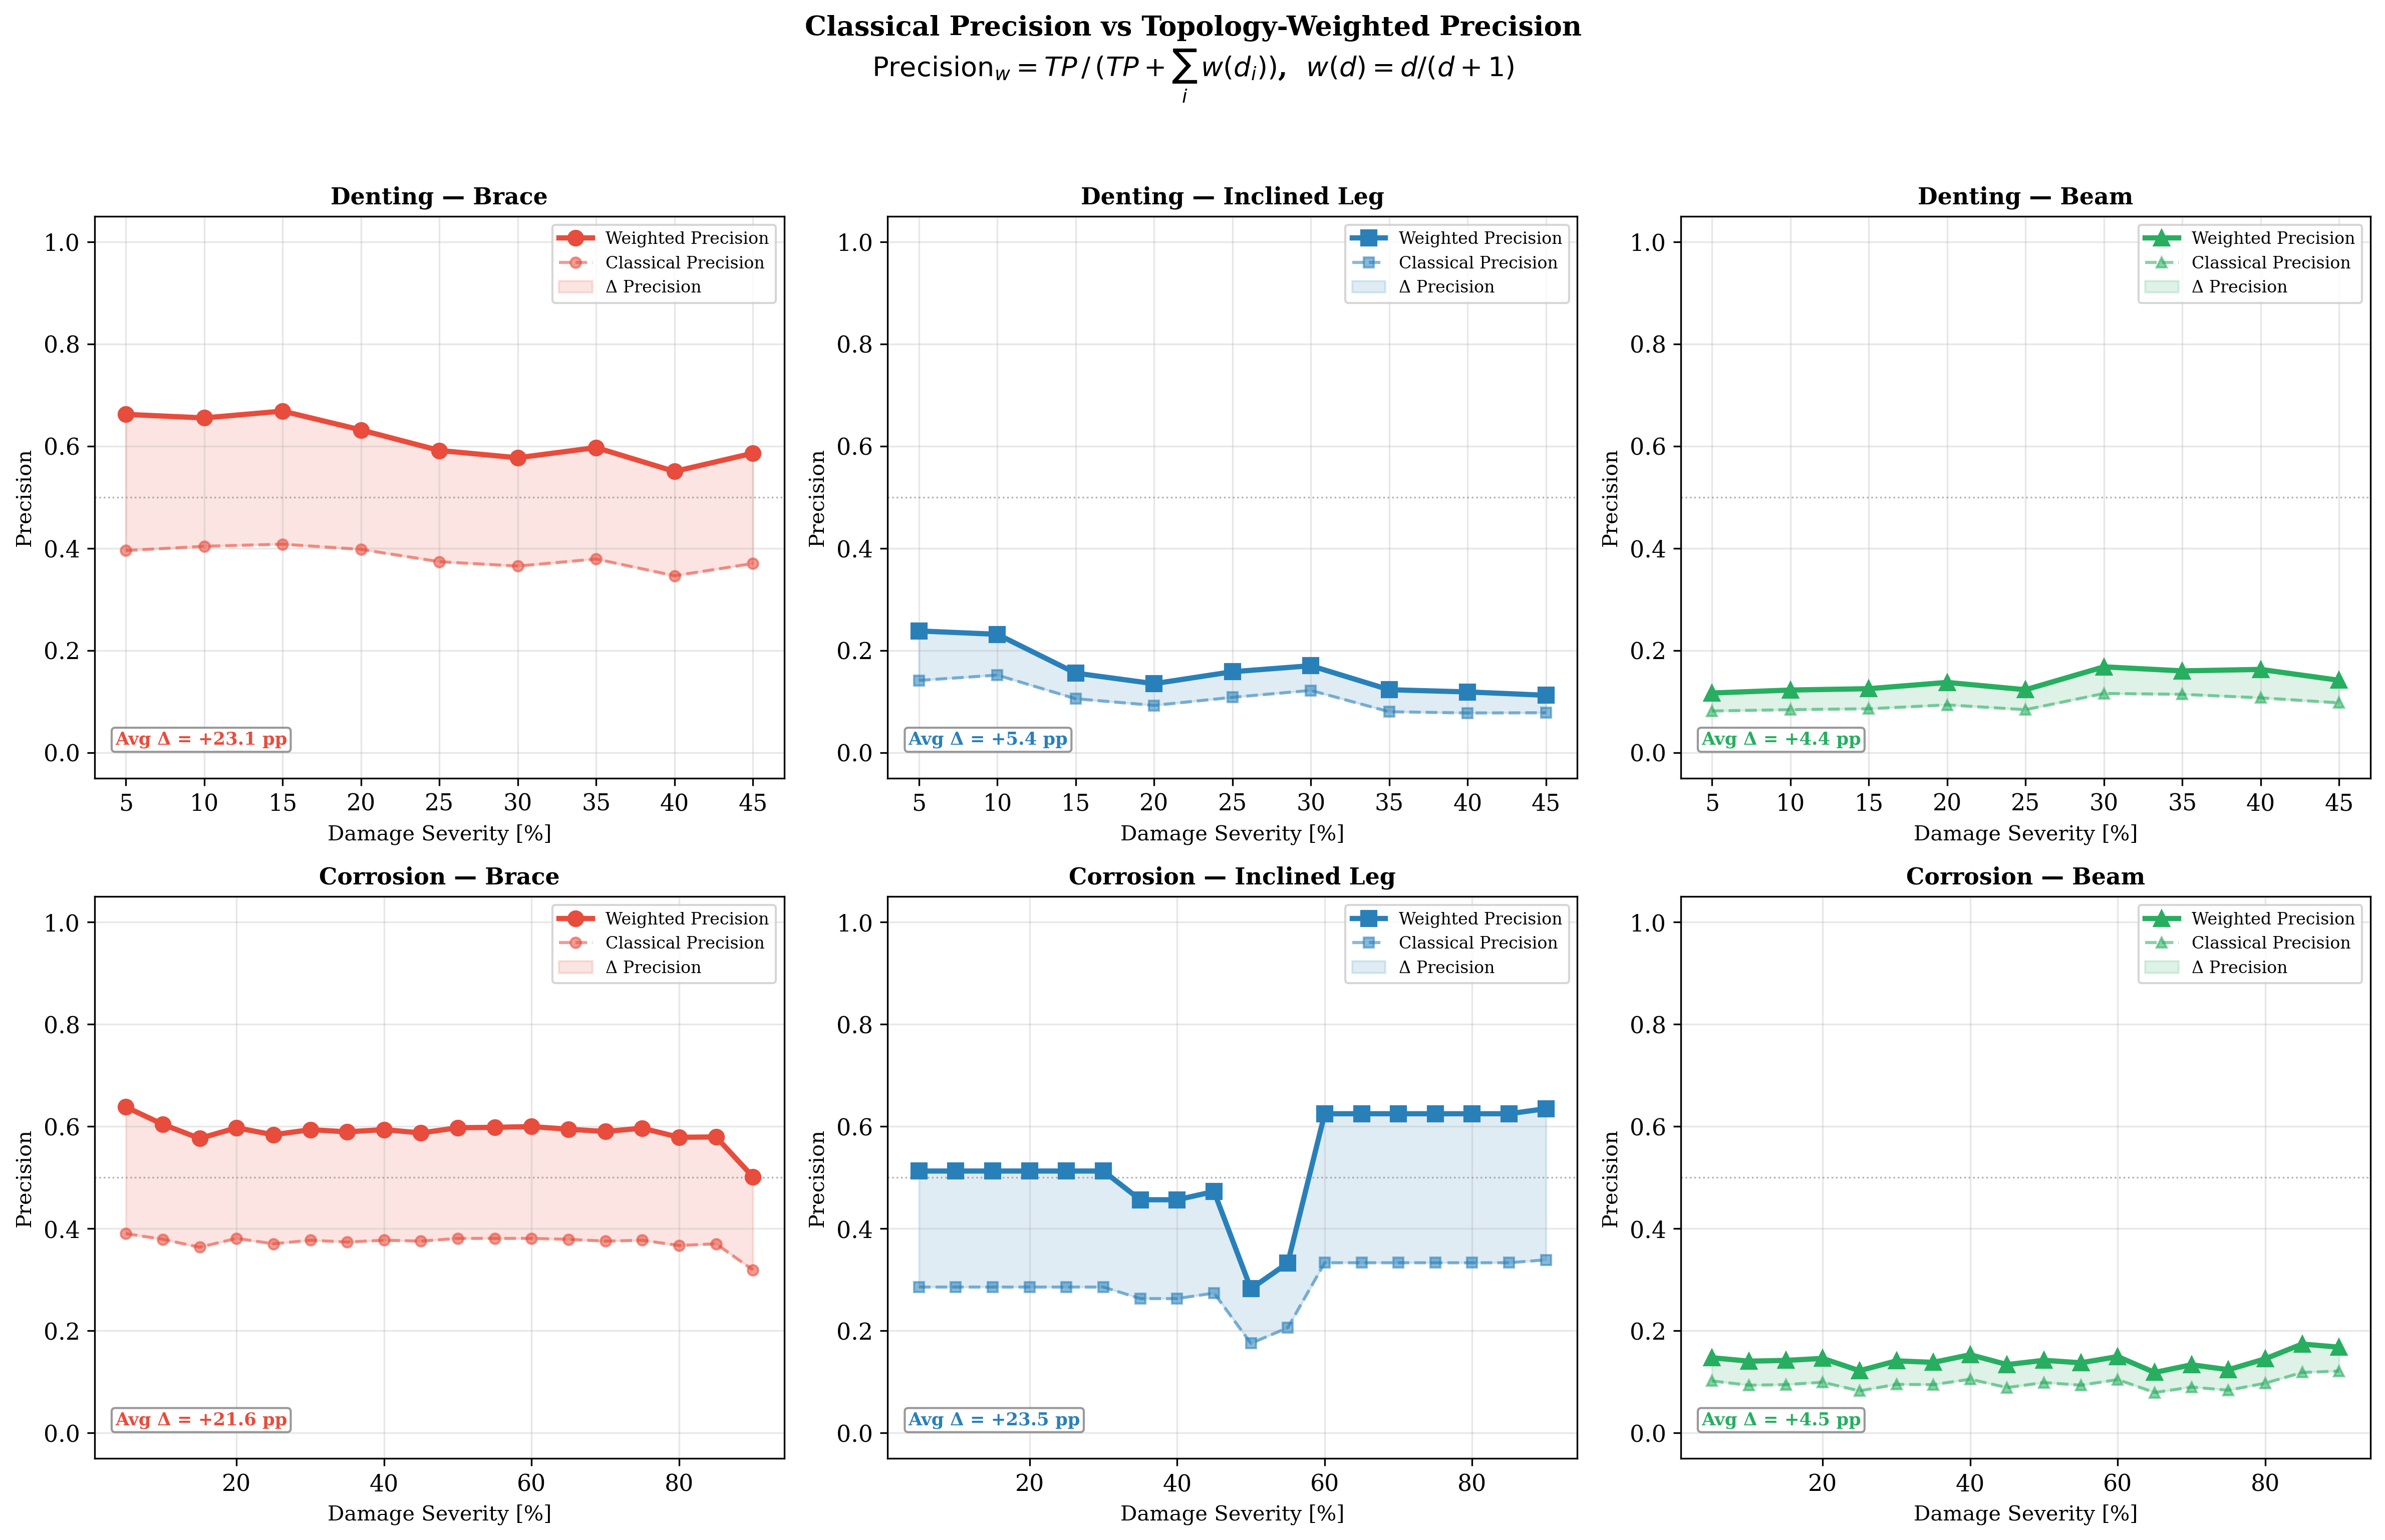
\includegraphics[width=0.9\textwidth]{../outputs/resultados_nuevos/Precision_clasica_vs_ponderada_por_elemento.png}
    \caption{Evolution of Classical Precision (dashed line) and Topology-Weighted Precision (solid line) as a function of damage severity.}
    \label{fig:precision_vs_severidad}
\end{figure*}

Table~\ref{tab:precision_ponderada} (Appendix~\ref{sec:apendice}) reports the complete numerical values by scenario, element type, and severity, including the mean FP distance.

% ─────────────────────────────────────────────────────────────────────────────
% §4.7  ROBUSTNESS TO GAUSSIAN NOISE
% ─────────────────────────────────────────────────────────────────────────────
\subsection{Robustness to Gaussian Noise (SNR)}
\label{subsec:SNR}

To evaluate the applicability of the method under realistic measurement conditions, controlled additive Gaussian noise with SNR levels between 5 and 50~dB was injected into the modal vectors prior to DQI evaluation. Figure~\ref{fig:SNR_degradation} shows the AUC-ROC degradation as a function of SNR level for the three element types.

\begin{figure*}[!t]
    \centering
    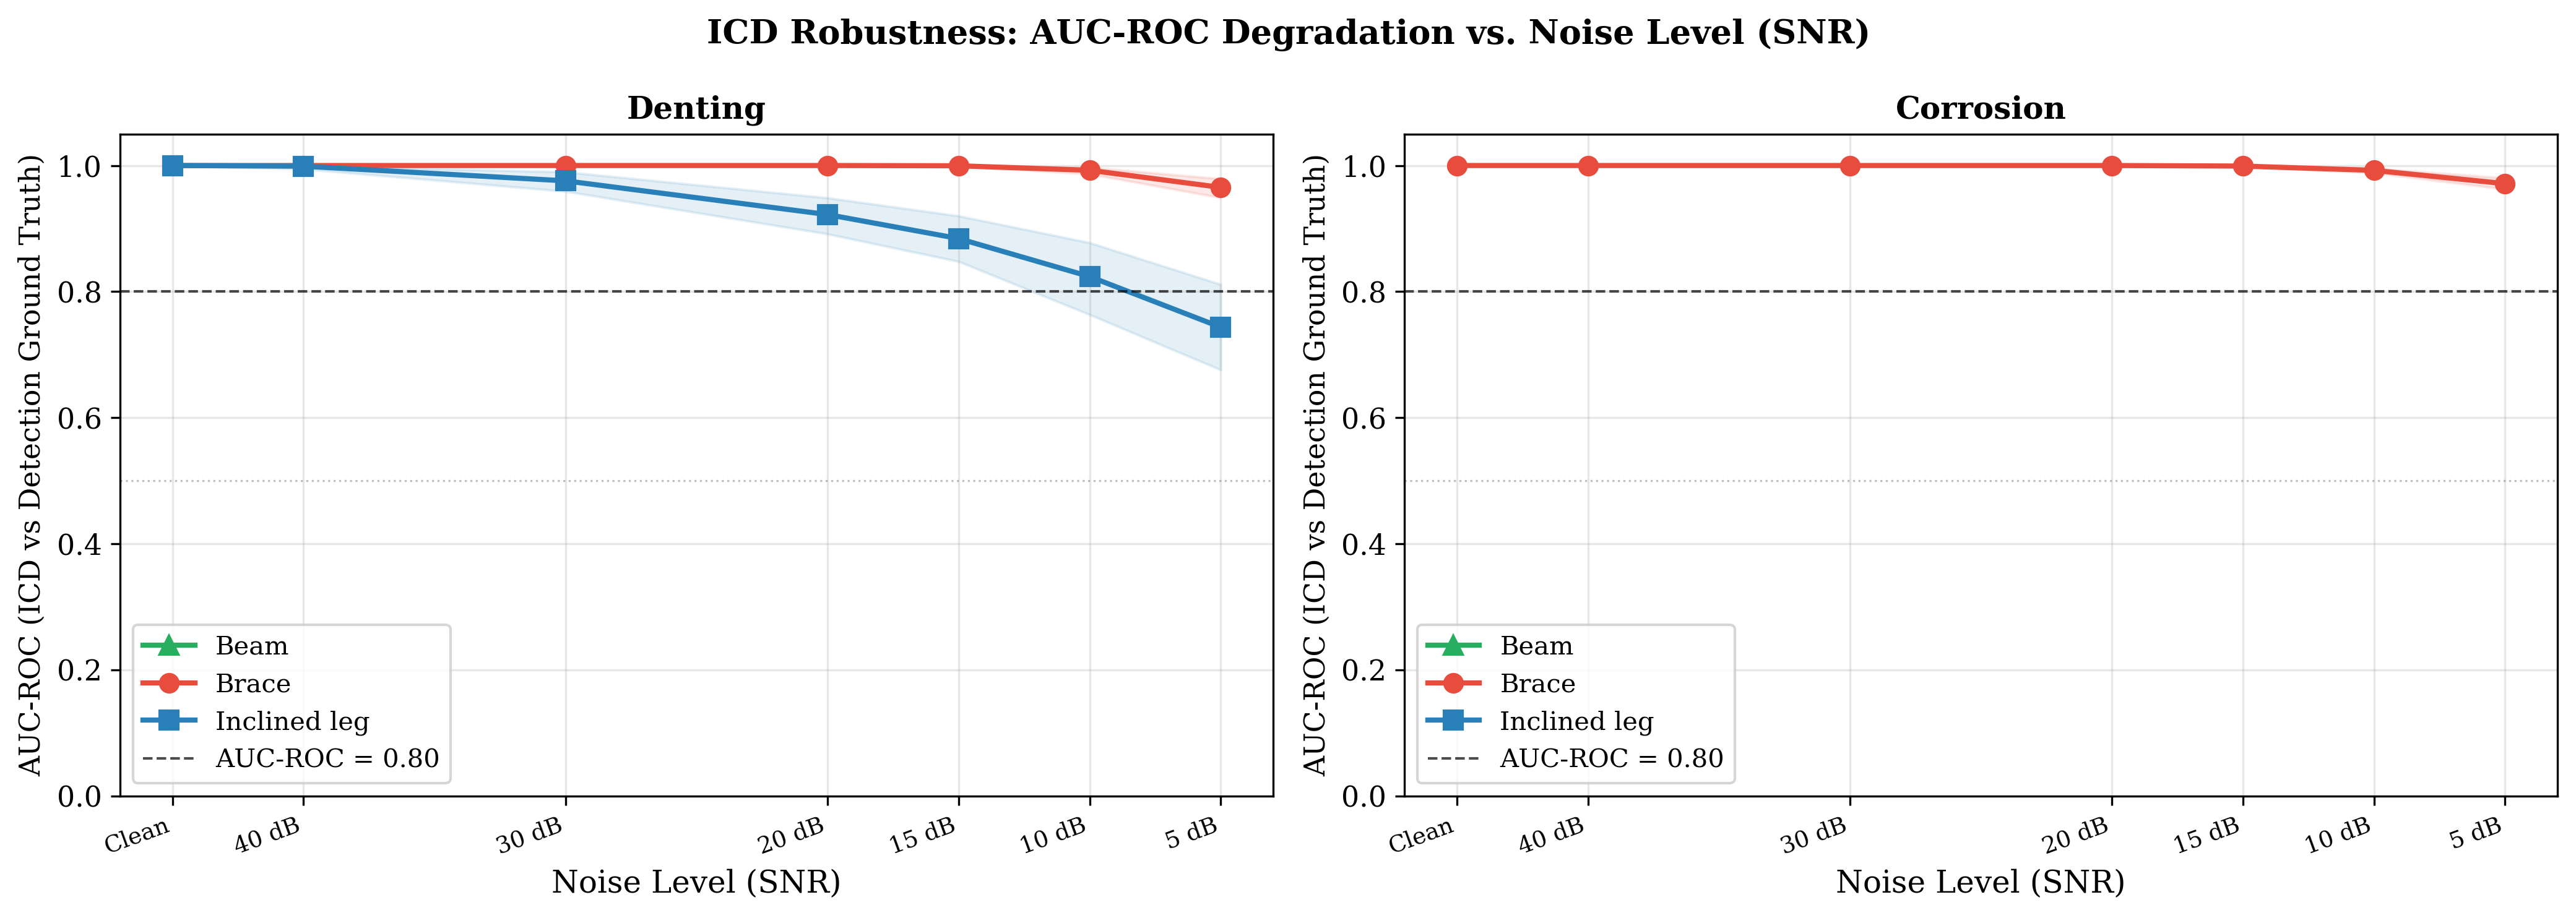
\includegraphics[width=0.9\textwidth]{../outputs/resultados_nuevos/AUC_ROC_vs_SNR_degradation.png}
    \caption{AUC-ROC degradation as a function of noise level (SNR) for Denting (left)
             and Corrosion (right). Dashed line = AUC~$=$ 0.80 threshold.}
    \label{fig:SNR_degradation}
\end{figure*}

The results demonstrate that the DQI maintains AUC-ROC~$> 0.80$ up to noise levels of
SNR~$= 20$~dB for braces, corresponding to moderately noisy measurement conditions typical
of MEMS systems installed on operating offshore platforms. Table~\ref{tab:snr_robustness}
summarises the AUC-ROC values at key SNR points.

\clearpage
\begin{table*}[!ht]
  \centering
  \caption{AUC-ROC of the DQI framework under additive white Gaussian noise (AWGN) at decreasing SNR levels. Ground truth: strict criterion (\texttt{DeteccionOK}=1.0). Monte Carlo estimation with $N_{\text{MC}}=500$ repetitions per SNR level.}
  \label{tab:snr_robustness}
  \begin{tabular}{llccccc}
    \toprule
    Damage & Member & \multicolumn{4}{c}{AUC-ROC at SNR level} & Degradation \\
    Type & Type & Clean & 20~dB & 10~dB & 5~dB & Clean$\to$5~dB \\
    \midrule
    Denting & Beam & N/A$^*$ & N/A$^*$ & N/A$^*$ & N/A$^*$ & N/A$^*$ \\
     & Brace & 1.000 & 1.000 & 0.992 & 0.965 & +3.5\% \\
     & Inclined Leg & 0.966 & 0.964 & 0.947 & 0.912 & +5.6\% \\
    \midrule
    Corrosion & Beam & N/A$^*$ & N/A$^*$ & N/A$^*$ & N/A$^*$ & N/A$^*$ \\
     & Brace & 1.000 & 1.000 & 0.992 & 0.971 & +2.9\% \\
     & Inclined Leg & 0.969 & 0.965 & 0.947 & 0.911 & +6.0\% \\
    \bottomrule
  \end{tabular}
  \par\smallskip
  {\footnotesize\raggedright
  SNR: Signal-to-Noise Ratio in decibels. AUC-ROC: Area Under the Receiver
  Operating Characteristic curve (range [0.5, 1.0], higher is better).
  Degradation (\%): relative AUC-ROC loss from clean to 5~dB SNR.
  $^*$~N/A: AUC-ROC is undefined for Beam members because the DQI never achieves
  correct element localisation (\texttt{DeteccionOK}$=0.5$ in all Beam cases, i.e.,
  detection occurs but is attributed to the adjacent element). As discussed in
  Section~\ref{subsec:metricas_clasificacion}, this reflects the negligible modal strain
  energy stored by horizontal beams in the low-order bending modes rather than a numerical
  limitation, and is invariant to the penalisation parameter $\beta$.
  \par}
\end{table*}

\FloatBarrier
\subsection{Limitations and Scope of Validity}
\label{subsec:limitaciones}

The following modelling assumptions define the boundary conditions of validity of the results reported in this study:

\begin{enumerate}
    \item \textbf{Numerical validation only.} All experiments are conducted on a calibrated FE model; no field or laboratory measurement data are incorporated. The 3{,}240-run campaign provides statistical robustness within this numerical framework, but absolute DQI performance may differ in the presence of model-plant mismatch, spatially correlated sensor noise, or unmeasured operational loads.
    \item \textbf{Linear elastic behaviour.} The formulation assumes small displacements and linear material response. Scenarios involving plastic deformation, fatigue-induced non-linearity, or residual stresses fall outside the validated scope.
    \item \textbf{Perfect modal identification.} The DIs are computed from exact FE eigenvalues and eigenvectors. In practice, modal extraction from noisy acceleration records introduces identification uncertainty beyond the additive Gaussian noise model of Section~\ref{subsec:SNR}.
    \item \textbf{Single-element damage.} Each GA run targets one damaged element. The behaviour of the DQI under simultaneous multi-element damage---a realistic scenario in advanced corrosion---has not been assessed.
    \item \textbf{Platform-specific topological calibration.} The decay constant $\beta$ is calibrated to the BFS neighbourhood of this platform (Equation~\ref{eq:beta_calibration}); structures with substantially different node connectivity require recalibration, although Equation~\ref{eq:beta_calibration} provides a direct, structure-independent protocol for doing so.
\end{enumerate}

\section{Conclusions and Future Work}
\label{sec:conclusiones}

This study has validated the effectiveness of the Detection Quality Index (DQI) as a robust metric for structural damage identification in jacket-type offshore platforms. The adopted approach extends the GA-based DI combination framework introduced by Ervin and Zeng~\citep{ervin2022index} to the offshore jacket domain, incorporating the DQI as the fitness function. Unlike the original binary target vector, the DQI exponentially penalises false positives and weights damage severity. This extension, together with the statistical validation over 3{,}240 scenarios, constitutes the central methodological contribution of the work. The campaign of 3{,}240 runs (1{,}080 denting $+$ 2{,}160 corrosion) on 120 ETABS model elements provides exhaustive statistical support for the reported results.

The most relevant finding confirms the behaviour of secondary members (diagonals or braces) as \emph{structural fuses}. The results demonstrate that the DQI is highly sensitive to damage in these elements, detecting stiffness reductions from 30\% severity (for both corrosion and denting) with global detection rates of \textbf{92.2\%} (denting) and \textbf{96.5\%} (corrosion), and AUC-ROC values exceeding 0.90 for the localisable member types (braces and inclined legs). By contrast, primary members (legs) exhibited significant redundancy, requiring damage levels above 50\% to become detectable by the system. This has a direct operational implication for offshore integrity management: while vibration-based automated monitoring is well-suited to the continuous surveillance of braces, underwater visual inspections should continue to prioritise main nodes and legs, where modal changes are more subtle in early stages.

A Gaussian noise robustness analysis demonstrates that the AUC-ROC remains above 0.80 up to an SNR level of 20~dB for braces, which is consistent with the measurement conditions of MEMS systems installed on operating platforms.

As a novel methodological contribution, the \textbf{Topology-Weighted Precision} ($\text{Precision}_w$) is proposed. This metric corrects the uniform penalisation of FPs by assigning a weight $w(d) = d/(d+1)$ based on their distance in the structural graph. The analysis shows that approximately 40\% of FP nodes are adjacent to the damaged element ($d = 1$), implying that classical Precision systematically underestimates localisation quality. The new metric raises brace Precision by up to \textbf{$+$22 percentage points}, providing a fairer assessment of localiser performance in structural networks.

Furthermore, the DQI formulation proved effective in penalising false positives---a critical attribute for avoiding unnecessary alarms that increase operational costs in offshore facilities.

\subsection{Future Work}

To consolidate the industrial applicability of this method, the following research directions are proposed:

\begin{itemize}
    \item \textbf{Experimental Validation:} Apply the methodology to vibration data from MEMS sensor arrays installed on operating jacket platforms \citep{ghsoub2018structural} or to laboratory-scale replica structures subjected to controlled corrosion immersion or impact testing. The critical quantities to characterise are: (i)~the performance gap between the idealised Gaussian noise model (Section~\ref{subsec:SNR}) and operational noise, which typically includes correlated wave and current excitation; (ii)~the effect of incomplete modal identification on the eight DIs; and (iii)~empirical validation of the $D=0.5$ partial-credit criterion for adjacent-element detections against actual structural response measurements.
    \item \textbf{Environmental and Operational Uncertainty:} Incorporate non-stationary environmental inputs---irregular wave sequences modelled by JONSWAP spectra, variable current profiles, and deck load fluctuations---as upstream disturbances to the modal identification step, evaluating whether the DQI's Gaussian noise robustness extends to correlated, non-white excitation conditions representative of the offshore operational environment.
    \item \textbf{Multi-Element and Progressive Damage:} Extend the GA framework to simultaneously localise and quantify damage in multiple structural members, addressing scenarios of advanced corrosion where several braces may be degraded concurrently. A multi-target DQI formulation would require redefining the localisation success factor $D$ for vector-valued damage scenarios and evaluating the interaction between overlapping BFS neighbourhoods.
    \item \textbf{Normative Integration:} Investigate how DQI-based detection confidence could be incorporated into risk-informed inspection planning frameworks aligned with current standards such as ISO~19902 and API RP~2SIM, with the objective of formally quantifying the reduction in underwater inspection frequency achievable through continuous vibration-based monitoring.
\end{itemize}

%% ─────────────────────────────────────────────────────────────────
%% APPENDIX
%% ─────────────────────────────────────────────────────────────────
\appendix
\section{Supplementary Tables}
\label{sec:apendice}

\onecolumn
\begin{longtable}{llrrrrr}
  \caption{Comparison of Classical and Topology-Weighted Precision. $\Delta$ = Weighted $-$ Classical (percentage points). Avg FP dist: mean topological distance (in structural members) between false-positive nodes and the damaged element. Weight function: $w(d)=d/(d+1)$.}\label{tab:precision_ponderada} \\
  \toprule
  Type & Element & Sev.[\%] & Prec.\ Cl. & Prec.\ Wgt. & $\Delta$ [pp] & FP dist \\
  \midrule
  \endfirsthead
  \multicolumn{7}{c}{\small\textit{Table continued from previous page}} \\[2pt]
  \toprule
  Type & Element & Sev.[\%] & Prec.\ Cl. & Prec.\ Wgt. & $\Delta$ [pp] & FP dist \\
  \midrule
  \endhead
  \midrule
  \multicolumn{7}{r}{\small\textit{Continued on next page}} \\
  \endfoot
  \bottomrule
  \endlastfoot
    Denting & Brace & 5 & 0.396 & 0.662 & +26.7 & 2.20 \\
    Denting & Brace & 10 & 0.404 & 0.655 & +25.1 & 2.16 \\
    Denting & Brace & 15 & 0.408 & 0.669 & +26.1 & 2.07 \\
    Denting & Brace & 20 & 0.398 & 0.632 & +23.4 & 4.40 \\
    Denting & Brace & 25 & 0.374 & 0.592 & +21.8 & 4.09 \\
    Denting & Brace & 30 & 0.365 & 0.577 & +21.2 & 4.01 \\
    Denting & Brace & 35 & 0.379 & 0.597 & +21.8 & 4.22 \\
    Denting & Brace & 40 & 0.346 & 0.551 & +20.4 & 3.66 \\
    Denting & Brace & 45 & 0.370 & 0.586 & +21.6 & 4.04 \\
    \cmidrule{2-7}
    Denting & Inclined Leg & 5 & 0.142 & 0.238 & +9.7 & 1.51 \\
    Denting & Inclined Leg & 10 & 0.152 & 0.232 & +8.0 & 1.52 \\
    Denting & Inclined Leg & 15 & 0.106 & 0.156 & +5.0 & 1.71 \\
    Denting & Inclined Leg & 20 & 0.093 & 0.135 & +4.3 & 1.73 \\
    Denting & Inclined Leg & 25 & 0.108 & 0.159 & +5.0 & 1.59 \\
    Denting & Inclined Leg & 30 & 0.122 & 0.170 & +4.8 & 1.57 \\
    Denting & Inclined Leg & 35 & 0.080 & 0.123 & +4.3 & 1.70 \\
    Denting & Inclined Leg & 40 & 0.078 & 0.119 & +4.1 & 1.74 \\
    Denting & Inclined Leg & 45 & 0.078 & 0.112 & +3.4 & 1.79 \\
    \cmidrule{2-7}
    Denting & Beam & 5 & 0.082 & 0.117 & +3.5 & 1.70 \\
    Denting & Beam & 10 & 0.084 & 0.123 & +3.8 & 1.71 \\
    Denting & Beam & 15 & 0.086 & 0.125 & +3.9 & 1.60 \\
    Denting & Beam & 20 & 0.094 & 0.138 & +4.4 & 1.47 \\
    Denting & Beam & 25 & 0.084 & 0.123 & +3.9 & 1.58 \\
    Denting & Beam & 30 & 0.116 & 0.168 & +5.2 & 1.45 \\
    Denting & Beam & 35 & 0.114 & 0.160 & +4.6 & 1.48 \\
    Denting & Beam & 40 & 0.107 & 0.163 & +5.6 & 1.38 \\
    Denting & Beam & 45 & 0.098 & 0.142 & +4.4 & 1.47 \\
    \midrule
    Corrosion & Brace & 5 & 0.390 & 0.638 & +24.8 & 2.89 \\
    Corrosion & Brace & 10 & 0.379 & 0.604 & +22.5 & 3.14 \\
    Corrosion & Brace & 15 & 0.364 & 0.577 & +21.3 & 3.13 \\
    Corrosion & Brace & 20 & 0.381 & 0.597 & +21.7 & 3.37 \\
    Corrosion & Brace & 25 & 0.370 & 0.584 & +21.3 & 3.24 \\
    Corrosion & Brace & 30 & 0.377 & 0.594 & +21.6 & 3.30 \\
    Corrosion & Brace & 35 & 0.374 & 0.590 & +21.6 & 3.32 \\
    Corrosion & Brace & 40 & 0.377 & 0.594 & +21.7 & 3.37 \\
    Corrosion & Brace & 45 & 0.376 & 0.587 & +21.2 & 2.89 \\
    Corrosion & Brace & 50 & 0.381 & 0.598 & +21.7 & 3.25 \\
    Corrosion & Brace & 55 & 0.381 & 0.598 & +21.7 & 3.26 \\
    Corrosion & Brace & 60 & 0.381 & 0.600 & +21.9 & 3.22 \\
    Corrosion & Brace & 65 & 0.379 & 0.595 & +21.6 & 3.27 \\
    Corrosion & Brace & 70 & 0.376 & 0.590 & +21.5 & 4.31 \\
    Corrosion & Brace & 75 & 0.377 & 0.597 & +21.9 & 4.21 \\
    Corrosion & Brace & 80 & 0.367 & 0.579 & +21.2 & 4.15 \\
    Corrosion & Brace & 85 & 0.370 & 0.580 & +20.9 & 3.68 \\
    Corrosion & Brace & 90 & 0.319 & 0.502 & +18.2 & 3.21 \\
    \cmidrule{2-7}
    Corrosion & Inclined Leg & 5 & 0.286 & 0.513 & +22.7 & 1.29 \\
    Corrosion & Inclined Leg & 10 & 0.286 & 0.513 & +22.7 & 1.29 \\
    Corrosion & Inclined Leg & 15 & 0.286 & 0.513 & +22.7 & 1.29 \\
    Corrosion & Inclined Leg & 20 & 0.286 & 0.513 & +22.7 & 1.29 \\
    Corrosion & Inclined Leg & 25 & 0.286 & 0.513 & +22.7 & 1.29 \\
    Corrosion & Inclined Leg & 30 & 0.286 & 0.513 & +22.7 & 1.29 \\
    Corrosion & Inclined Leg & 35 & 0.263 & 0.457 & +19.3 & 1.39 \\
    Corrosion & Inclined Leg & 40 & 0.263 & 0.457 & +19.3 & 1.39 \\
    Corrosion & Inclined Leg & 45 & 0.274 & 0.473 & +19.9 & 1.44 \\
    Corrosion & Inclined Leg & 50 & 0.175 & 0.282 & +10.7 & 1.38 \\
    Corrosion & Inclined Leg & 55 & 0.206 & 0.333 & +12.7 & 1.60 \\
    Corrosion & Inclined Leg & 60 & 0.333 & 0.625 & +29.2 & 1.00 \\
    Corrosion & Inclined Leg & 65 & 0.333 & 0.625 & +29.2 & 1.00 \\
    Corrosion & Inclined Leg & 70 & 0.333 & 0.625 & +29.2 & 1.00 \\
    Corrosion & Inclined Leg & 75 & 0.333 & 0.625 & +29.2 & 1.00 \\
    Corrosion & Inclined Leg & 80 & 0.333 & 0.625 & +29.2 & 1.00 \\
    Corrosion & Inclined Leg & 85 & 0.333 & 0.625 & +29.2 & 1.00 \\
    Corrosion & Inclined Leg & 90 & 0.339 & 0.635 & +29.6 & 1.00 \\
    \cmidrule{2-7}
    Corrosion & Beam & 5 & 0.102 & 0.147 & +4.5 & 1.43 \\
    Corrosion & Beam & 10 & 0.094 & 0.141 & +4.7 & 1.38 \\
    Corrosion & Beam & 15 & 0.095 & 0.142 & +4.7 & 1.34 \\
    Corrosion & Beam & 20 & 0.099 & 0.146 & +4.7 & 1.38 \\
    Corrosion & Beam & 25 & 0.082 & 0.122 & +4.0 & 1.49 \\
    Corrosion & Beam & 30 & 0.095 & 0.141 & +4.6 & 1.45 \\
    Corrosion & Beam & 35 & 0.095 & 0.138 & +4.4 & 1.38 \\
    Corrosion & Beam & 40 & 0.105 & 0.153 & +4.8 & 1.38 \\
    Corrosion & Beam & 45 & 0.089 & 0.134 & +4.5 & 1.43 \\
    Corrosion & Beam & 50 & 0.099 & 0.142 & +4.4 & 1.47 \\
    Corrosion & Beam & 55 & 0.094 & 0.138 & +4.4 & 1.46 \\
    Corrosion & Beam & 60 & 0.105 & 0.150 & +4.5 & 1.44 \\
    Corrosion & Beam & 65 & 0.079 & 0.119 & +3.9 & 1.44 \\
    Corrosion & Beam & 70 & 0.090 & 0.134 & +4.4 & 1.45 \\
    Corrosion & Beam & 75 & 0.084 & 0.124 & +4.0 & 1.47 \\
    Corrosion & Beam & 80 & 0.098 & 0.145 & +4.8 & 1.40 \\
    Corrosion & Beam & 85 & 0.119 & 0.174 & +5.6 & 1.37 \\
    Corrosion & Beam & 90 & 0.121 & 0.168 & +4.7 & 1.49 \\
\end{longtable}
\twocolumn

%% ─────────────────────────────────────────────────────────────────
\bibliographystyle{cas-model2-names}
\bibliography{refs}

\end{document}
